% This template was written by John Davies <john.davies@glasgow.ac.uk> 2017-02-06
% It matches the university specification at the time of writing
%   for the widths of the page margins and one-and-a-half line spacing
% You may want to include more packages, particularly for heavy mathematics
% Please let me know if you find any errors or wish to suggest improvements

\documentclass[12pt,titlepage,oneside]{book}
\usepackage[T1]{fontenc} % modern encoding
% Comment out the next three lines of LaTeX if you wish to use Computer Modern fonts
%   (this is the default for LaTeX)
% Make sure that your TeX installation can produce good pdf with these fonts.
% The following three lines are a good alternative if you don't use much mathematics
\usepackage{mathptmx}  % uses Times for text and mathematics
\usepackage[scaled]{helvet} %  helvetica for sanserif, scaled 95% by default
\usepackage{courier}  % courier for typewriter font, pretty ugly but available
% otherwise the stix package offers more options and symbols
% \usepackage{stix}  % uses Times for text and a range of fonts for mathematics
% End of choices for fonts
\usepackage{graphicx}  % standard package for importing graphics files
\usepackage{cite}  % improves format of numerical citations, such as [1-3]
\usepackage[top=1.8cm, bottom=1.8cm,left=4.0cm,right=1.5cm]{geometry}
% These margins are the university guidelines
\usepackage[onehalfspacing]{setspace}  % gives one-and-a-half line spacing
% doublespacing is another option and can be changed in the text
\usepackage{dcolumn}   % needed for some tables
\usepackage{bm}        % for math
\usepackage{amssymb}   % for math
\usepackage{amsmath}
\usepackage{color}
\usepackage{acronym}
\usepackage{algcompatible}
\usepackage{newfloat}
\usepackage{cancel}
\usepackage{subcaption}
\graphicspath{{./figures/}}

\DeclareFloatingEnvironment[
    fileext=loa,
    listname=List of Algorithms,
    name=ALGORITHM,
    placement=tbhp,
]{algorithm}

\begin{document}
\begin{titlepage}
\centering
\vspace*{3cm}  % Need the * or the space is swallowed at the top of the page
\bfseries\Large
Data Analysis Techniques for Continuous Gravitational Wave Searches\\
\vspace{3cm}
\normalfont\large
Joseph Bayley\\
\vspace{2cm}
Submitted in fulfilment of the requirements for the\\
Degree of Doctor of Philosophy\\
\vspace{2cm}
School of Physics and Astronomy\\
College of Science and Engineering\\
University of Glasgow\\
\vspace{1cm}

\includegraphics[scale=0.125]{GlaLogo.pdf}
\\
\vspace{1cm}
% Insert month and year of date deposited with library for final version
February 2017
\end{titlepage}
\frontmatter  % Turn off chapter numbering, use roman page numbers
\chapter{Abstract}

The field of gravitational wave astronomy is still in its early stages, with
detections of compact binary coalescences numbering $\sim
12$ and the most recent observing run (O3) providing $\sim 50$ more candidates. Another possible source of
gravitational waves is rapidly rotating neutron stars which can emit gravitational waves if they have some asymmetry
around their rotation axis.
These are predicted to emit long duration quasi-sinusoidal signals known as
continuous gravitational waves.

% SOAP chapter
All-sky and wide parameter space searches for continuous gravitational waves
are generally template-matching schemes which test a bank of signal waveforms
against data from a gravitational wave detector.  Often these searches  are highly-tuned to specific signal types and are computationally
expensive. We have developed a search method (entitled SOAP) based on the Viterbi
algorithm which is model-agnostic and has a computational cost several orders
of magnitude lower than template methods and with a comparable sensitivity. 
In particular, this method can search for
signals which have an unknown frequency evolution. We test the algorithm on
three simulated and real data sets: gapless Gaussian noise, Gaussian noise with
gaps and real data from the final run of initial LIGO (S6). We show that at
95\% efficiency, with a 1\% false alarm rate, the algorithm achieves a sensitivity of $\sim 60,\, 72$ and $74$ in the optimal coherent signal to noise ratio in each of these datasets.
We discuss the use of this algorithm for detecting a wide range of quasi-monochromatic
gravitational wave signals and instrumental artefacts, and
demonstrate that it can also identify shorter duration signals such as compact binary coalescences.


% Machine learning chapter
Many continuous gravitational wave searches are affected by instrumental lines
as the long duration narrowband nature of a line can appear to be very similar
to a real continuous gravitational wave signal.  This has led
to the development of techniques to try and limit the effect of
instrumental lines, which mostly involve developing a statistic to penalise
signals that appear in only a single detector.  
Whilst these statistics limit the effect of instrumental lines, in the SOAP search described above, many lines still contaminated the statistics and had to be manually removed by investigating other search outputs.
We have developed a method using convolutional neural networks to reduce the impact of instrumental
artefacts on the SOAP search described above.  This has the
ability to identify features in each detectors spectrograms such that a
frequency band can be classified into a signal or noise class.  
This limits the amount of manual investigation of bands and allowed the SOAP search to be fully automated without a reduction in the sensitivity.



% Parameter est chapter 
Once a continuous gravitational wave is detected, we would want to extract some
parameters associated with the source to help understand more about its
structure and evolution. We describe a Bayesian method which extracts the sky
location, frequency, frequency derivative and signal to noise ratio of a source associated with the
frequency evolution returned by the SOAP algorithm.  This has the aim of
limiting the size of the parameter space for a more sensitive fully coherent
follow up search.  
We tested this approach on 200 simulations in Gaussian noise, and in 90\% of these simulations we limit the sky area to 45 deg$^2$ with a 95\% confidence contour.
However, find that this contour contains the true parameter only 42\% of the time.
We present these results and describe the features and shortcomings of our approach.

~\chris{You maybe don't need to
be as bluntly negative and honest as you are here. I would advise slightly
expanding the description but also say that we present results and describe the
features and shortcomings of our approach. Or something like that. While we are
talimng about the PE, I would expect the results to be more presentable if you
take the 50\% confindence interval as opposed to the 95\%. Have you been bale
to do this yet?}

% Lines chapter
As mentioned above, we limit the effect of instrumental lines on the SOAP
search using machine learning, however we can also identify and mitigate these
lines separately before a search is run.  We demonstrate how we can use SOAP in
a simple configuration to identify instrumental lines.  We compare this method
to existing line identification tools used in the \gls{LIGO} collaboration, and
find that using the Viterbi statistic SOAP identifies $\sim 37$\% of the same lines as these methods, where of the lines which were not identified, other SOAP outputs do show evidence of a line.
With further investigation, we expect to identify many more lines in common with existing methods.
As well as these common lines, the SOAP algorithm returned $\sim 150$ more bands which potentially contain an instrumental line, which did not appear on \gls{LIGO} line-lists.









\tableofcontents
\listoftables
\listoffigures
\chapter{Acknowledgements}


\chapter{Declaration}



\acrodef{GW}[GW]{gravitational-wave}
\acrodef{CW}[CW]{continuous wave}
\acrodef{NS}[NS]{neutron star}
\acrodef{EM}[EM]{electromagnetic}
\acrodef{SNR}[SNR]{signal-to-noise-ratio}
\acrodef{LIGO}[LIGO]{Laser Interferometer Gravitational-wave Observatory}
\acrodef{SFT}[SFT]{short Fourier transform}
\acrodef{UCD}[UCD]{up, centre or down}
\acrodef{MDC}[MDC]{mock data challenge}
\acrodef{PSD}[PSD]{power spectral density}
\acrodef{ROC}[ROC]{receiver operating characteristic}
\acrodef{RMS}[RMS]{root median square}
\acrodef{MCMC}[MCMC]{Markov-Chain Monte Carlo}

\mainmatter % Turn on chapter numbering, reset page numbers, use arabic
\chapter{\label{intro}Introduction}
%%%%%


\Glspl{GW} were first predicted in 1915 as a consequence of Einstein's general theory of relativity \citep{einstein2005GrundlageAllgemeinen}.
They are theorised as ripples in the fabric of space-time.
The first observational evidence that \glspl{GW} exist came from observations of the Hulse-Taylor binary \citep{weisberg1981GravitationalWaves,weisberg2004RelativisticBinary}. 
This observation of a pulsar in a binary system showed that the periastron was reached slightly early after each orbit, implying that the pulsars orbit was decreasing with time. 
If the separation of two orbiting objects is decreasing then the system must be losing energy.
The loss in energy matched the \gls{GR} prediction which assumed the energy was lost to \glspl{GW}.
This gave hope of \glspl{GW} existence and helped lead the way to designing instruments which could directly detect them.
The first direct detection of gravitational waves was made in 2015 when the two \gls{LIGO} detectors in the US \citep{abbott2016ObservationGravitational} identified a signal from a \gls{BBH} system.
This was not only the first observation of a \gls{GW} but gave information on a yet unobserved astrophysical system.
This has since been followed by many more detections of \gls{BBH} signals involving \gls{LIGO} and Virgo including \citep{abbott2017GW170814ThreeDetector,theligoscientificcollaboration2020GW190425Observation}.
In 2017 the \gls{LIGO} detectors observed the first \gls{BNS} system \citep{abbott2017GW170817Observation} which had a corresponding electromagnetic counterpart.
This allowed verification of the source from optical counterparts and started the era of multi-messenger astronomy.
These detections opened up the field of gravitational wave astronomy, where many more detections are expected to give more information on the universe and objects within it.

As well as searching for \gls{BBH} and \gls{BNS} signals, there are many efforts to detector other types of \gls{GW} signals. 
This thesis focuses on efforts to search for a particular type of \gls{GW} which are thought to originate from rapidly rotating neutron stars.
In chapters \ref{intro} and \ref{searchcw} I will review introductory material. 
This includes a general introduction to the generation of \glspl{GW} in Sec.~\ref{intro:gravwaves} and their sources in Sec.~\ref{intro:sources}.
I will then introduce instruments used to detect \gls{GW} in Sec.~\ref{intro:detector}.
In Chapter \ref{searchcw} I will introduce the general model for \glspl{CW} and current methods used to detect them.
Chapters \ref{soap}, \ref{machine} and \ref{detchar} will go into detail about techniques developed by the author to search for \gls{CW} signals. 
Finally I will summarise this work and discuss future developments in chapter \ref{summary}.


%%%%%%%%%%%
%%%%%%%%%
\section{\label{intro:gravwaves}Gravitational waves}
%%%%%%%%%%%
%%%%%%%%%

In general relativity, gravity is thought of as the curvature of space-time and matter moves according to this curvature. 
The matter in the universe also has an effect on the curvature of the space-time.
The larger the mass of matter the more the space-time is distorted.
Space-time can generally be described by Einstein's field equations
\begin{equation}
\label{intro:gravwaves:efe}
    G_{\mu \nu} = \frac{8 \pi G}{c^4}T_{\mu \nu}.
\end{equation}
where $G_{\mu \nu}$ is the Einstein tensor and $T_{\mu \nu}$ is the stress-energy tensor.
The stress energy tensor describes the mass-energy in the universe, where its components contain information on the density of energy and momentum.
The Einstein tensor contains information on the curvature of the universe. 
This can be derived directly from the metric tensor $g_{\mu \nu}$ which describes the geometry of the universe.
Einstein's equations then explain how the curvature of space-time changes with the mass-energy within it. 
In empty space one can assume that the geometry of space-time is flat, i.e. there is no curvature to space-time. The metric tensor for this can then be defined as
\begin{equation}
g_{\mu \nu} = \eta_{\mu \nu} = \left(
\begin{matrix}
-1 & 0 & 0 & 0 \\
0 & 1 & 0 & 0 \\
0 & 0 & 1 & 0 \\
0 & 0 & 0 & 1 
\end{matrix}
\right).
\end{equation}
Each index of this matrix refers to a space-time dimension, i.e. $x^0 = t$, $x^1=x$, $x^2=y$ and $x^3=z$. 
Measuring a distance $dx$ in space-time can be different for different observers, therefore, one needs a measure which is invariant for every observer. 
This is the space-time interval $ds$, also known as the line element, between two `events' in space-time. 
This is defined as
\begin{equation}
\label{intro:lineelement}
    ds^2 = g_{\mu \nu} dx^{\mu}dx^{\nu}.
\end{equation}
As in Einstein's notation this is a sum over the indices $\mu$ and $\nu$.  
Equation \ref{intro:lineelement} can be thought to describe the space-time `distance' between the two events.
For flat space-time, $\eta_{\mu\nu}$, this can then be written as
%
\begin{equation}
    ds^2 = -c^2 dt^2 + dx^2 + dy^2 + dz^2.
\end{equation}
%
The Einstein equations Eq.~\ref{intro:gravwaves:efe} then demonstrate how the curvature of space-time $G_{\mu\nu}$ depends on the matter and energy distribution $T_{\mu \nu}$ within it.

A gravitational wave can be described as a ripple in this space time.
The simplest way to visualise this is just a small time dependent change to the flat space-time metric $\eta_{\mu\nu}$.
In linearised theory of gravity, the space-time metric $g_{\mu \nu}$ can be defined as
\begin{equation}
\label{intro:gravwave:metric}
    g_{\mu \nu} = \eta_{\mu \nu} + h_{\mu \nu},
\end{equation}
where $ \eta_{\mu \nu}$ is the metric for flat space-time and $h_{\mu \nu}$ is some perturbation, where $|h_{\mu \nu}| \ll 1$ \citep{flanagan2005BasicsGravitational}. 
In this linearised theory the perturbations to the metric tensor are assumed to be small, therefore, Einstein's field equations can be solved such that the solution is a plane wave. 
More information on this derivation can be found in \citep{flanagan2005BasicsGravitational,letiec2016TheoryGravitational}.
By using $g_{\mu \nu}$ from Eq.~\ref{intro:gravwave:metric}, we can write the linearised Einstein equations as
\begin{equation}
\label{intro:lineinstein}
    \Box h_{\mu \nu} = -16 \pi T_{\mu\nu},
\end{equation}
where $\Box$ is the d'Alembert operator which in flat space is defined by
\begin{equation}
		\Box = -\frac{1}{c^2} \frac{\partial^2}{\partial t^2} + \frac{\partial^2}{\partial x^2} + \frac{\partial^2}{\partial y^2} + \frac{\partial^2}{\partial z^2}
\end{equation}
In empty space there is no matter, therefore, all the components of the stress energy tensor  are zero, i.e. $T_{\mu \nu} = 0$.
This allows Eq.~\ref{intro:lineinstein} to be reduced to
\begin{equation}
    \Box h_{\mu \nu} = 0,
\end{equation}
Which is of course the wave equation. 
This follows the same form as in electrodynamics and the general plane-wave solutions have the form
\begin{equation}
    h_{\mu\nu} = A_{\mu\nu}e^{ik_{\alpha} x^{\alpha}},
\end{equation}
where each component of $h_{\mu \nu}$ is a sinusoid traveling along vector $k_{\alpha}$ with amplitude $A_{\mu\nu}$ \citep{capano2011SearchingGravitational}.
At this point the set of equations are not simple; the symmetric tensor $A_{\mu \nu}$ has 10 independent components.
This can be greatly simplified by choosing a different gauge where the metric perturbation is both transverse and traceless (TT) \citep{flanagan2005BasicsGravitational}.
This is just a choice of coordinate system which does not change any current assumptions \joe{read more about gauges}. A traceless metric is one where the sum of the diagonal elements are 0 and a transverse metric is when the oscillations are perpendicular to the direction of travel. 
This gauge imposes two conditions: one is that $h_{\mu \nu}$ is traceless, i.e. that the sum of the diagonal elements are 0 and the other is that $h_{\mu \nu}$ is transverse. 
The transverse element means that the oscillations of the wave happen perpendicular to the direction of travel.
At this point we can choose that the wave is traveling in the $z$ direction which means that $k = (\omega,0,0,k)$.
By then adopting the TT gauge there are only two unique components to the metric such that the perturbation is
\begin{equation}
\label{intro:gw:gravwave}
h_{\mu \nu} = \left( 
\begin{matrix}
0 & 0 & 0 & 0 \\
0 & h_{+} & h_{\times} & 0 \\
0 & h_{\times} & -h_{+} & 0 \\
0 & 0 & 0 & 1 \\
\end{matrix}
\right) 
e^{i(kt - wt)}.
\end{equation}
The two unique components are then the two polarisations of gravitational waves, $h_{+}$ and $h_{\times}$.
The affect of each of the polarisations on a ring of test particles can be seen in Fig.~\ref{gw:polarisations} where the gravitational wave is travelling out of the page.

\begin{figure}[h]
    \centering
    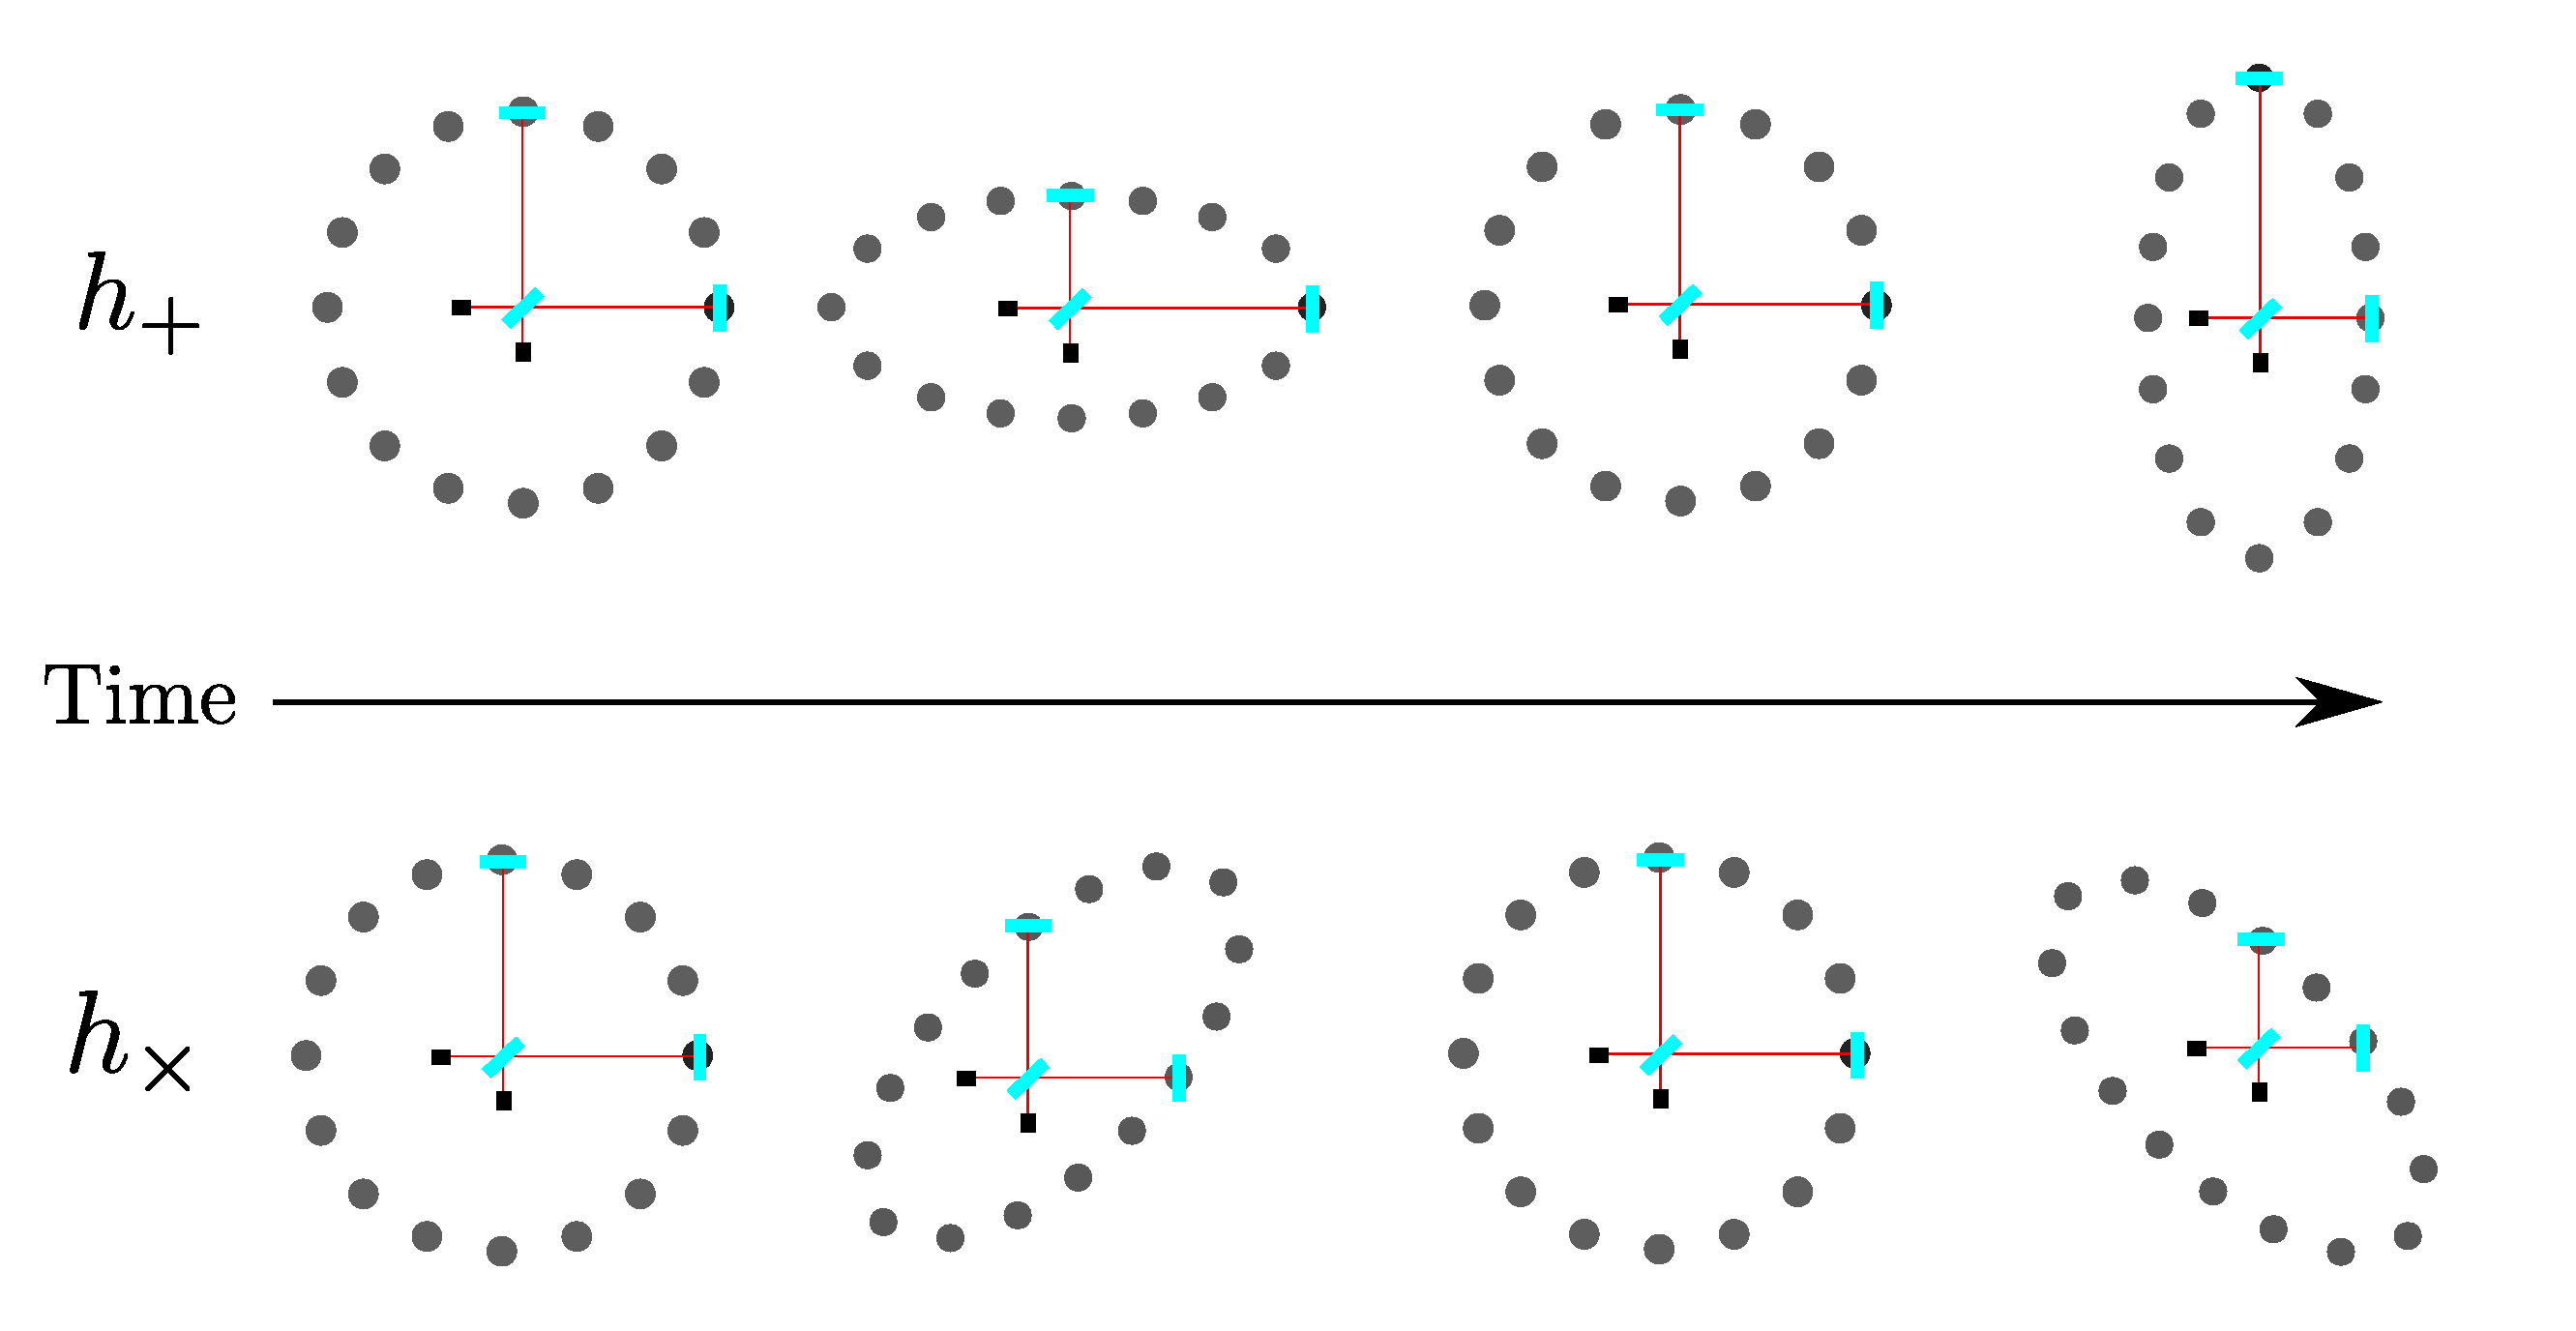
\includegraphics[width=\textwidth]{C1_intro/polarisation_ring.pdf}
    \caption[Plus and Cross polarisations]{Shows how the plus and cross polarisations affect a ring of test particles. This assumes the wave is travelling out of the page and the effects have been greatly exaggerated. This also shows an example of how this effects the test masses of an interferometer. This will be described in more detail in Sec.~\ref{intro:detector}.}
    \label{gw:polarisations}
\end{figure}



\subsubsection{Generating gravitational waves}

To generate gravitational waves we go back to Eq.~\ref{intro:lineinstein} where we include the stress-energy term on the right hand side.
Following the derivation in \citep{flanagan2005BasicsGravitational}, one can find that the gravitational wave amplitude is related to the second moment of the mass distribution.
The second moment of the mass distribution $I_{\mu\nu}$is defined as
\begin{equation}
    I_{\mu \nu}(t) = \int \rho(t,{\bf x}) x^\mu x^\nu d^3x,
\end{equation}
where $\rho$ is the mass density, and $x_i$ and $x_j$ are the coordinates \citep{flanagan2005BasicsGravitational}. 
This is the quadrupole moment tensor without the trace subtracted.
The gravitational wave amplitude is then
\begin{equation}
\label{intro:gravwave:amp}
    h_{\mu \nu} = \frac{2}{r}  \frac{d^2 I_{\mu \nu}(t-r)}{dt^2},
\end{equation}
where $r$ is the distance from the source \citep{letiec2016TheoryGravitational}.
This has a slight modification in the TT gauge, see \citep{flanagan2005BasicsGravitational}, however, has the same relationship between the mass quadrupole and the \gls{GW} amplitude.
This shows that for a \gls{GW} to be generated, the second derivative of the mass quadrupole moment is needed.
A mass quadrupole moment only exists when the mass distribution is not spherically symmetric.
Therefore, a mass which is asymmetric and accelerating will produce a \gls{GW}.

Systems which will produce detectable \glspl{GW} are generally rapidly rotating high mass systems which have some asymmetry around their rotation axis.
The sources of these \gls{GW} will be described in the following section.



%%%%%%%%%%%%%%
%%%%%%%%%%%%%
\section{\label{intro:sources}Sources and signals}
%%%%%%%%%%%%%%%
%%%%%%%%%%%%%%%

There are many potential sources for \gls{GW}. The expected sources can be split into 3 general categories based on their signal type: Transient, Stochastic and \glspl{CW}.
These categories are chosen based on the length of the signal and how well modelled the signal is.
Figure \ref{intro:sources:signaltypes} shows an example of each of the signals and their category.
%
\begin{figure}[h]
    \centering
    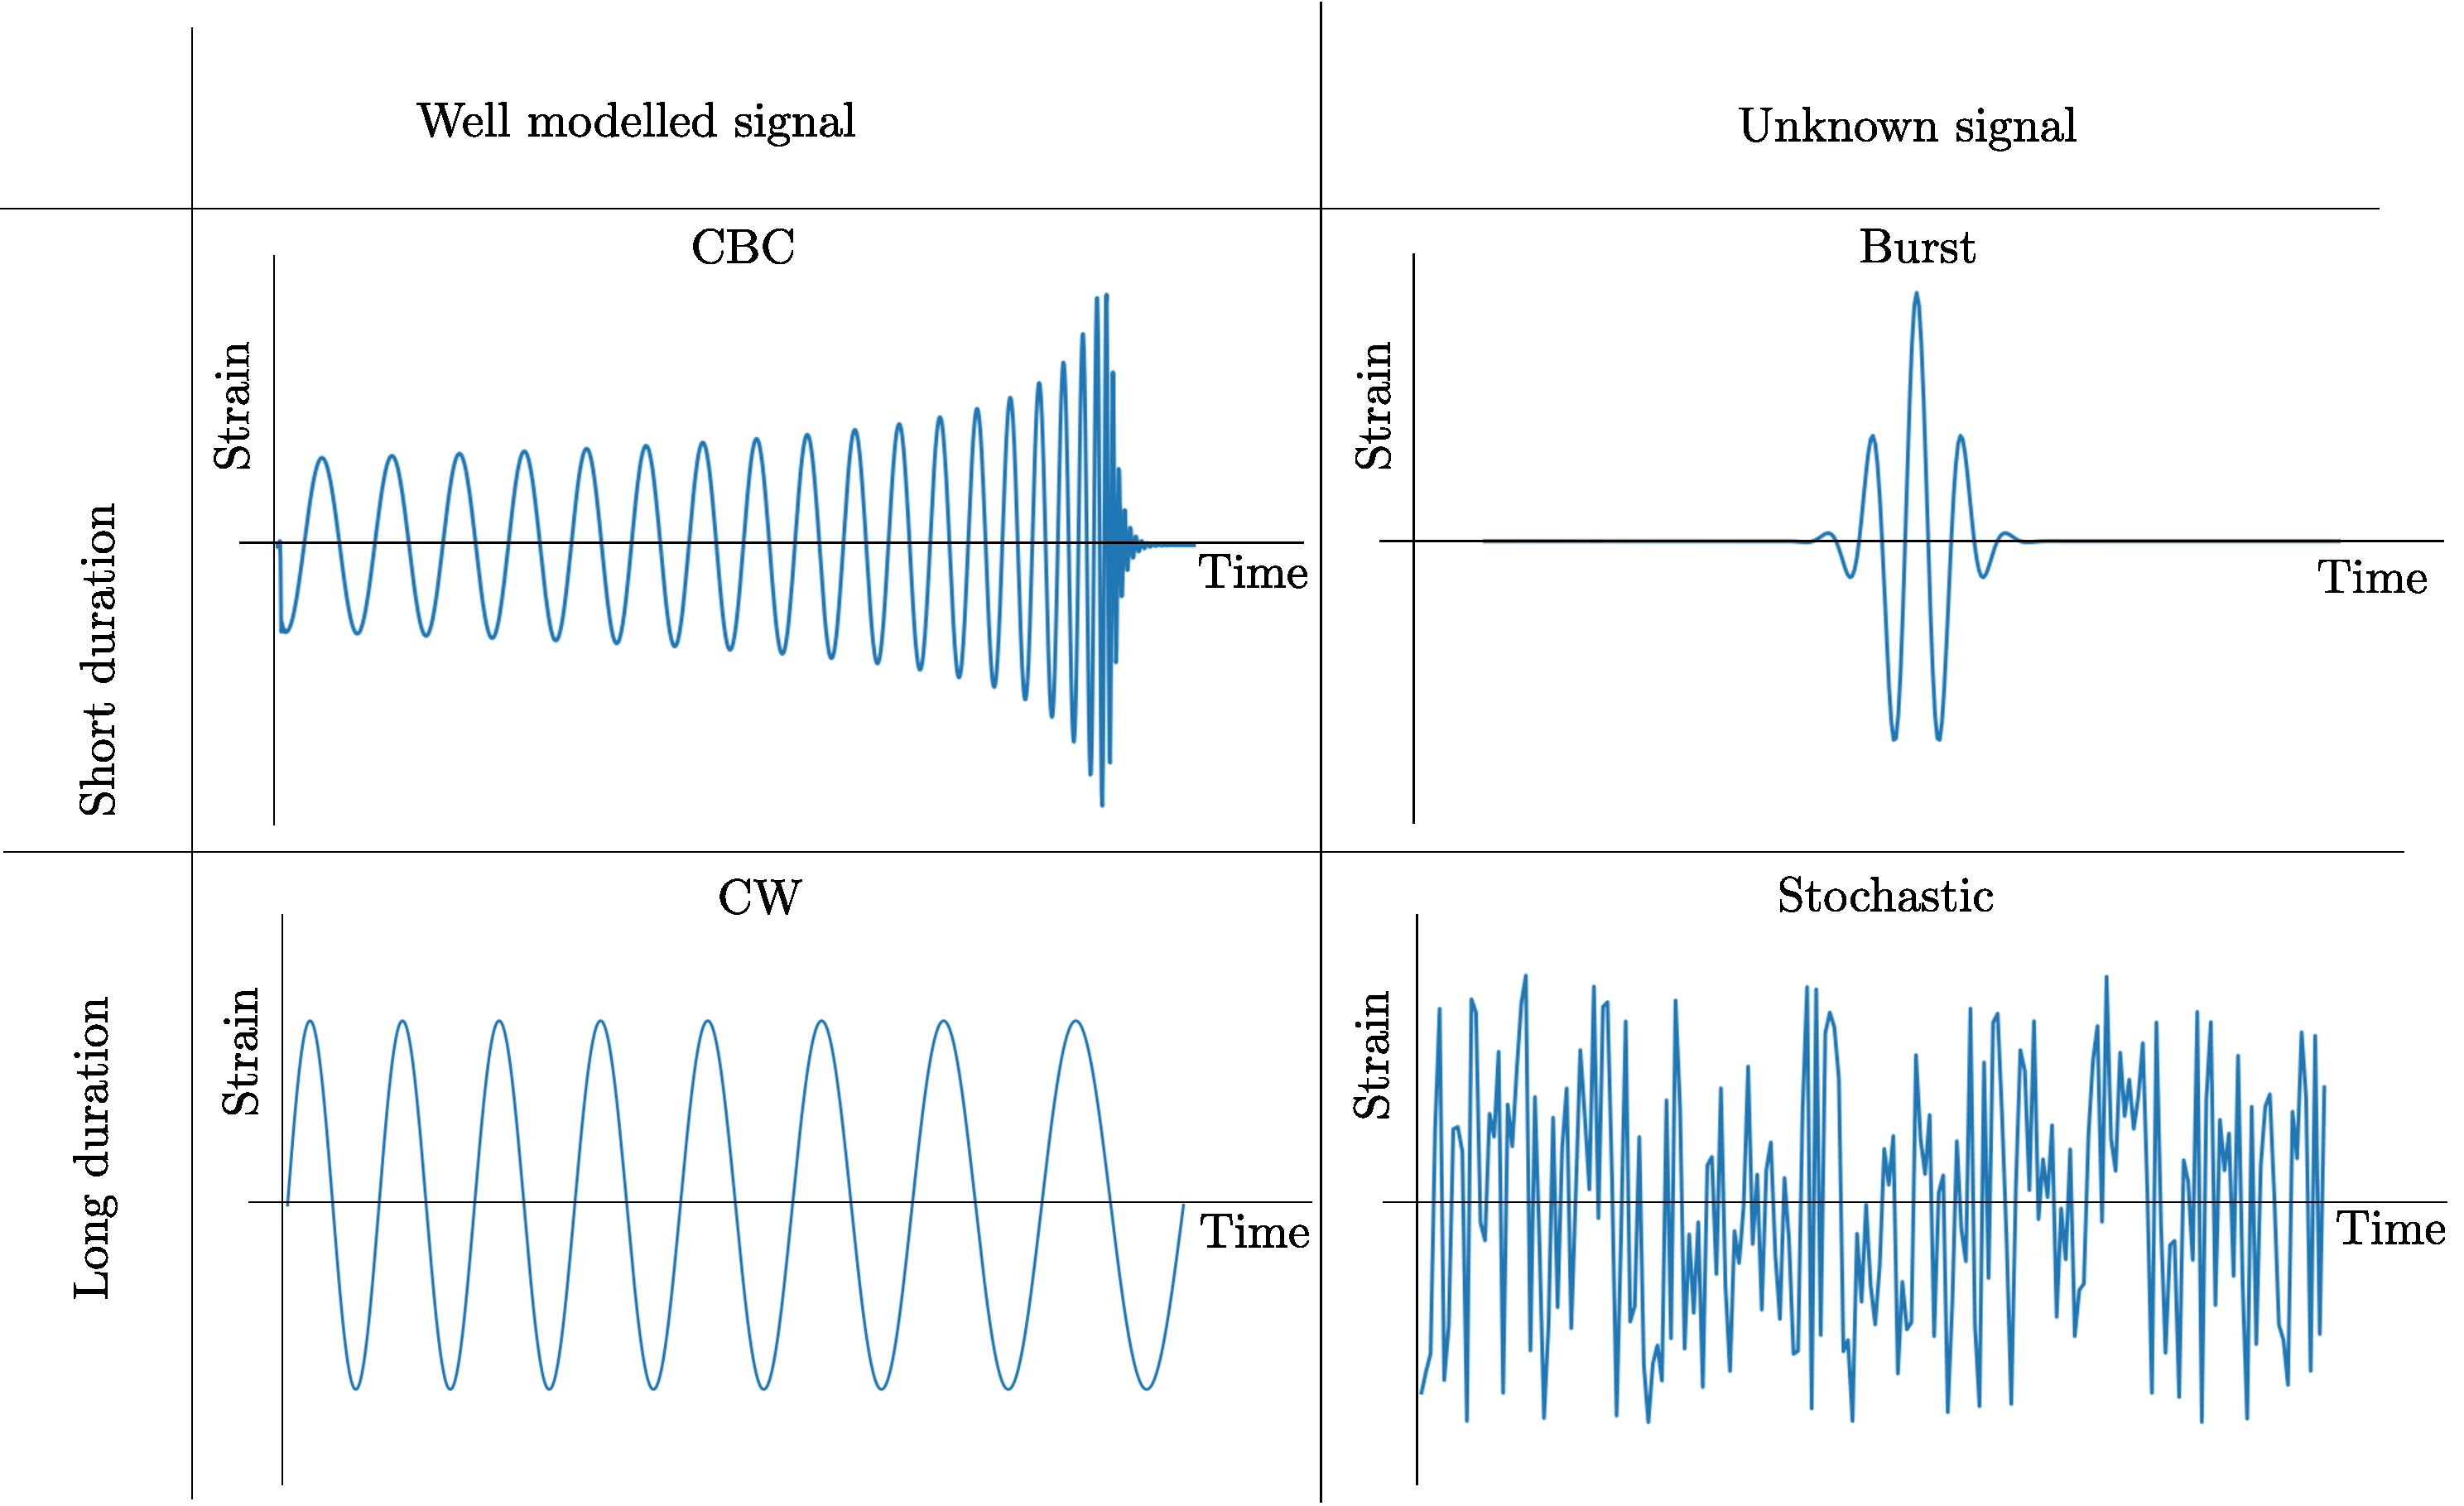
\includegraphics[width=\textwidth]{C1_intro/sources_types.pdf}
    \caption[GW signal types]{Each \gls{GW} signal type can be categorised based on its signal length and how well the signal is modelled. Transient signals which are short duration in the ground based detectors band, include both well modelled \gls{CBC} signals and unknown Burst signals. Long duration signals include well modelled \gls{CW} signals and unknown Stochastic signals.}
    \label{intro:sources:signaltypes}
\end{figure}
In the sections that follow, I will give an overview of the potential sources of each of these signal categories and their wave-forms.


%%%%%%%%%%%%%%%
\subsection{\label{sources:transient} Transient}
%%%%%%%%%%%%%%%

Transient sources of \glspl{GW} are short duration signals which are, depending on the source, observable from milliseconds to tens of seconds in current ground based detectors frequency band. 
Some of these sources, particularly \gls{CBC} sources, will emit signals for a much longer time, however these are at a lower frequency and not observable by current ground based detectors detectors.
Transient signals can be further split into two categories based on how well they are modelled. 
\glspl{CBC} have well modelled wave-forms and bursts are generally from un-modelled or unknown sources.

\subsubsection{\label{sources:transient:cbc} Compact Binary Coalescence}

\glspl{CBC} originate from the in-spiral and merge of two compact objects which are gravitationally bound.
The objects inspiral as they lost energy to the radiation of gravitational waves.
Dependent on the masses and distances of the two objects, the gravitational waves generated by the system can be detected by ground based detector such as LIGO \citep{aasi2015AdvancedLIGO} and Virgo \citep{acernese2015AdvancedVirgo}. 
In fact, the only detections to date have been of this type; these are summarised in \citep{ligoscientificcollaborationandvirgocollaboration2019GWTC1GravitationalWave}.

\joe{More qualatative, See Grahams comment}
The compact objects referred to here are either either black holes or neutron stars.
There are generally three types of \gls{CBC} source: \gls{BBH}, \gls{BNS} and \gls{NSBH}.
The general structure of the waveform is the same for each of these and follows a `chirp' where the \gls{GW} frequency increases with time until merger. An example of this is shown in Fig.~\ref{intro:sources:signaltypes}.
For higher mass systems such as \gls{BBH} these signals are detectable by ground based detectors for $< 1\,s$. 
For lower mass systems such as \gls{BNS} they can be detected for longer periods $\mathcal{O}(10)$s. 
The lower frequency parts of the signal (i.e. earlier times) aim to be detected by future space based detectors such as \gls{LISA} \citep{danzmann1996LISALaser}.

In systems which have a neutron star, during the in-spiral and merger phase, the neutron star can deform due tidal interactions between the objects \citep{flanagan2008ConstrainingNeutronstar}. 
This becomes useful as it will affect the generated waveform and can help place limits on and determine the \gls{EOS} for the dense matter in a neutron star \citep{harry2018ObservingMeasuring}. %\citep{hernandezvivanco2019MeasuringNeutron}
\gls{BNS} systems also offer a way do observe objects in multiple different channels, or what is known as multi-messenger astronomy. 
This is where the object can be viewed in the \gls{EM} spectrum as well as in gravitational waves.
This offers much in the field of astronomy as it can aid in the measurement of the Hubble constant \citep{theligoscientificcollaborationandthevirgocollaboration2017GravitationalwaveStandard}. 
Observations of \gls{BBH} systems can also give information on how black holes and \glspl{BBH} form, more details on this can be found in \citep{zevin2017ConstrainingFormation,mandel2018MergingStellarmass}.


%%%%%%%%%%%%%%
\subsubsection{\label{sources:transient:burst}Burst}
%%%%%%%%%%%%%%%%%

Burst sources are also short duration however, are un-modelled or difficult to model, in the sense that the exact waveform of the signal is unknown.
There are two possible reasons for the lack in knowledge of the waveform: the physics of the system is too complicated to model in a reasonable amount of time or there is no model of the source.
As there is no model to generate waveforms, burst searches cannot use matched filtering as in \gls{CBC} searches.
Rather burst searches look for short bursts in power which is coincident between multiple detectors \citep{cornish2015BayeswaveBayesian, klimenko2008CoherentMethod}.
There are a number of systems which could potentially emit a short duration burst signals.
These include core collapse supernovae \citep{ott2008GravitationalWave}, \glspl{GRB} \citep{aasi2014SearchGravitational}, cosmic strings \citep{damour2005GravitationalRadiation} and other unknown sources.
Detecting \gls{GW} from one of these sources could offer more insight into the processes which cause core collapse supernovae. 

As burst searches are un-modelled, they are sensitive to almost any signal which is coherent between detectors. 
This allows them to also search for signals from \gls{CBC} as well as any \gls{GW} signal from an unknown source.



%%%%%%%%%%%%%%%
\subsection{Stochastic}
%%%%%%%%%%%%%%%

The stochastic background has no signal model, however, is expected to be a persistent source of \gls{GW} in the background of the detector. 
The stochastic background is the incoherent sum of many unresolved \gls{GW} signals.
The source of these signals can be anything from cosmological sources such as cosmic strings to \gls{CBC} signals.
These signals can be thought of as the \gls{GW} analogue of the \gls{CMB}.
The signal is assumed to be isotropic such that it can be observed at any point on the sky \citep{christensen2018StochasticGravitational}. 
As the stochastic background is noise-like it is very difficult to distinguish from noise within a single detector \citep{christensen2018StochasticGravitational}.
Therefore, searches for the stochastic background correlate signals between multiple detectors \citep{romano2019SearchesStochastic,christensen2018StochasticGravitational}. 
When detected, these signals may be able to offer insights into the early universe and its formation.



%%%%%%%%%%%%%%%%%%
\subsection{\label{intro:sources:cw}Continuous waves}
%%%%%%%%%%%%%%%%%%%%

\glspl{CW} are long duration signals which can be well modelled.
The signals last for times greater than the observation runs of ground based detectors and in general have a fixed or slowly varying frequency.
There are a number or potential sources of \glspl{CW} including a \gls{CBC} signal earlier in the inspiral phase.
Before the final stages of the inspiral of a \gls{CBC} signal, the objects orbiting at much slower non-relativistic speeds. They therefore emit a \gls{GW} with a slowly varying frequency and can remain in this phase for millions of years. 
This signal however, is at lower frequency than ground based detectors can detect, therefore space based detectors such as \gls{LISA} \citep{danzmann1996LISALaser} are expected to observe this type of \gls{CW}.

The primary source for many \glspl{CW} searches is rapidly rotating neutron stars with spin periods ranging from $\sim 10^{-3} - 10$ s \citep{manchester2005AustraliaTelescope}.
Neutron stars originate when a massive star $\sim 11 - 20 M_{\odot}$ collapses and are the remnant of this collapse, they are objects with incredibly high density and are highly magnetised with field strengths of $10^8 - 10^{15}$ G \citep{konar2017MagneticFields}.
They have masses around $1.4-2 \; M_{\odot}$ contained in a star with radius of $\sim 10$ km.
Despite many observations in the electromagnetic spectrum and a large amount of research, these objects are not well understood.
A key part or neutron stars which is not understood is the \gls{EOS}. A review of the current understanding can be found in \cite{lattimer2016EquationState}.
The \gls{EOS} relates quantities such as the pressure and density of a neutron star and dictates how the neutron star matter behaves.
Observations of \glspl{GW} from neutron stars can place limits on the \gls{EOS} of this type of matter. 
These observations have already been made in the form of \gls{BNS} mergers \citep{abbott2017GW170817Observation}.
However, independent observations of rapidly rotating neutron stars can add to this understanding by placing limits on the deformability of the star and therefore the \gls{EOS}.

For a neutron star to emit a gravitational wave it needs to have some asymmetry in its mass distribution around its rotation axis, this follows from Eq.~\ref{intro:gravwave:amp}. 
There are a number of different mechanisms which could cause this and emit \glspl{GW}, some of these are reviewed in \citep{glampedakis2017GravitationalWaves,riles2017RecentSearches,haskell2015DetectingGravitational,lasky2015GravitationalWaves}.
Here I will summarise two main theories: Neutron star mountains and neutron star oscillations.


%%%%%%
\subsubsection{\label{intro:source:cw:mountain}Mountains}
%%%%%%%%%

One of more likely mechanisms for detectable \gls{GW} emission from neutron stars is from `mountains' on the surface of the star.
These are permanent deformations of the crust which are non axisymmetric, i.e. the deformation is not symmetric around the rotation axis.

This deformation or asymmetry can be quantified by the ellipticity $\epsilon$ of the neutron star.
This is defined using the principal moments of inertial
\begin{equation}
\label{ellipticity}
\epsilon = \frac{I_{xx}-I_{yy}}{I_{zz}},
\end{equation}
where $I_{zz},I_{xx},I_{yy}$ are the principal moment of inertia.
This is when the star is rotating around the $z$ axis so $I_{zz}$ is along the rotation axis. 

There are a number of theories which describe the origin of this axisymmetry.
If the pulsar is in a binary system and accreting material from its companion star, the material can be funneled towards the magnetic poles by the magnetic field, thereby causing a hot spot \citep{haskell2015DetectingGravitational}.
This `hot spot' could cause a deformation on the surface of the star which is not axisymmetric. 
The magnetic stresses from strong magnetic fields within the star, could potentially also cause non axisymmetric deformations to the star \citep{}.
Finally the spin down of the pulsar itself could cause stresses in the crust of the star until the point of breaking, its then after this break which could leave a distortion in the crust \citep{becker2009NeutronStars}.
More details on the signal waveform of this type of \gls{GW} and methods to search for it will be explained in Sec.~\ref{searchcw}.
 
 %%%%%%%%%%%%%%
 \subsubsection{Neutron star oscillations}
 %%%%%%%%%%%%%%%
 \joe{Probably shorten this section, as may not know enough to answer questions on}
There are a number of oscillation modes within a star such as f-modes, p-modes and r-modes \citep{becker2009NeutronStars}. 
Each of these waves are oscillations in the star similar to oscillations in the earth which measured in terrestrial seismology.
The difference between these modes is the restoring force bringing the perturbed state back to equilibrium.
For example, gravity is the restoring force for f-modes where the oscillations happen in the crust of the star.
The more promising of these for gravitational wave emission and detection is the r-mode \citep{lasky2015GravitationalWaves}. 
These are oscillations in the neutron superfluid part of the star, where the restoring force is the Coriolis effect from the rotation of the star.
Figure \ref{intro:source:cw:rmode} shows an highly exaggerated view of a neutron star with an oscillation mode travelling in each direction.
\begin{figure}[h]
	\centering
	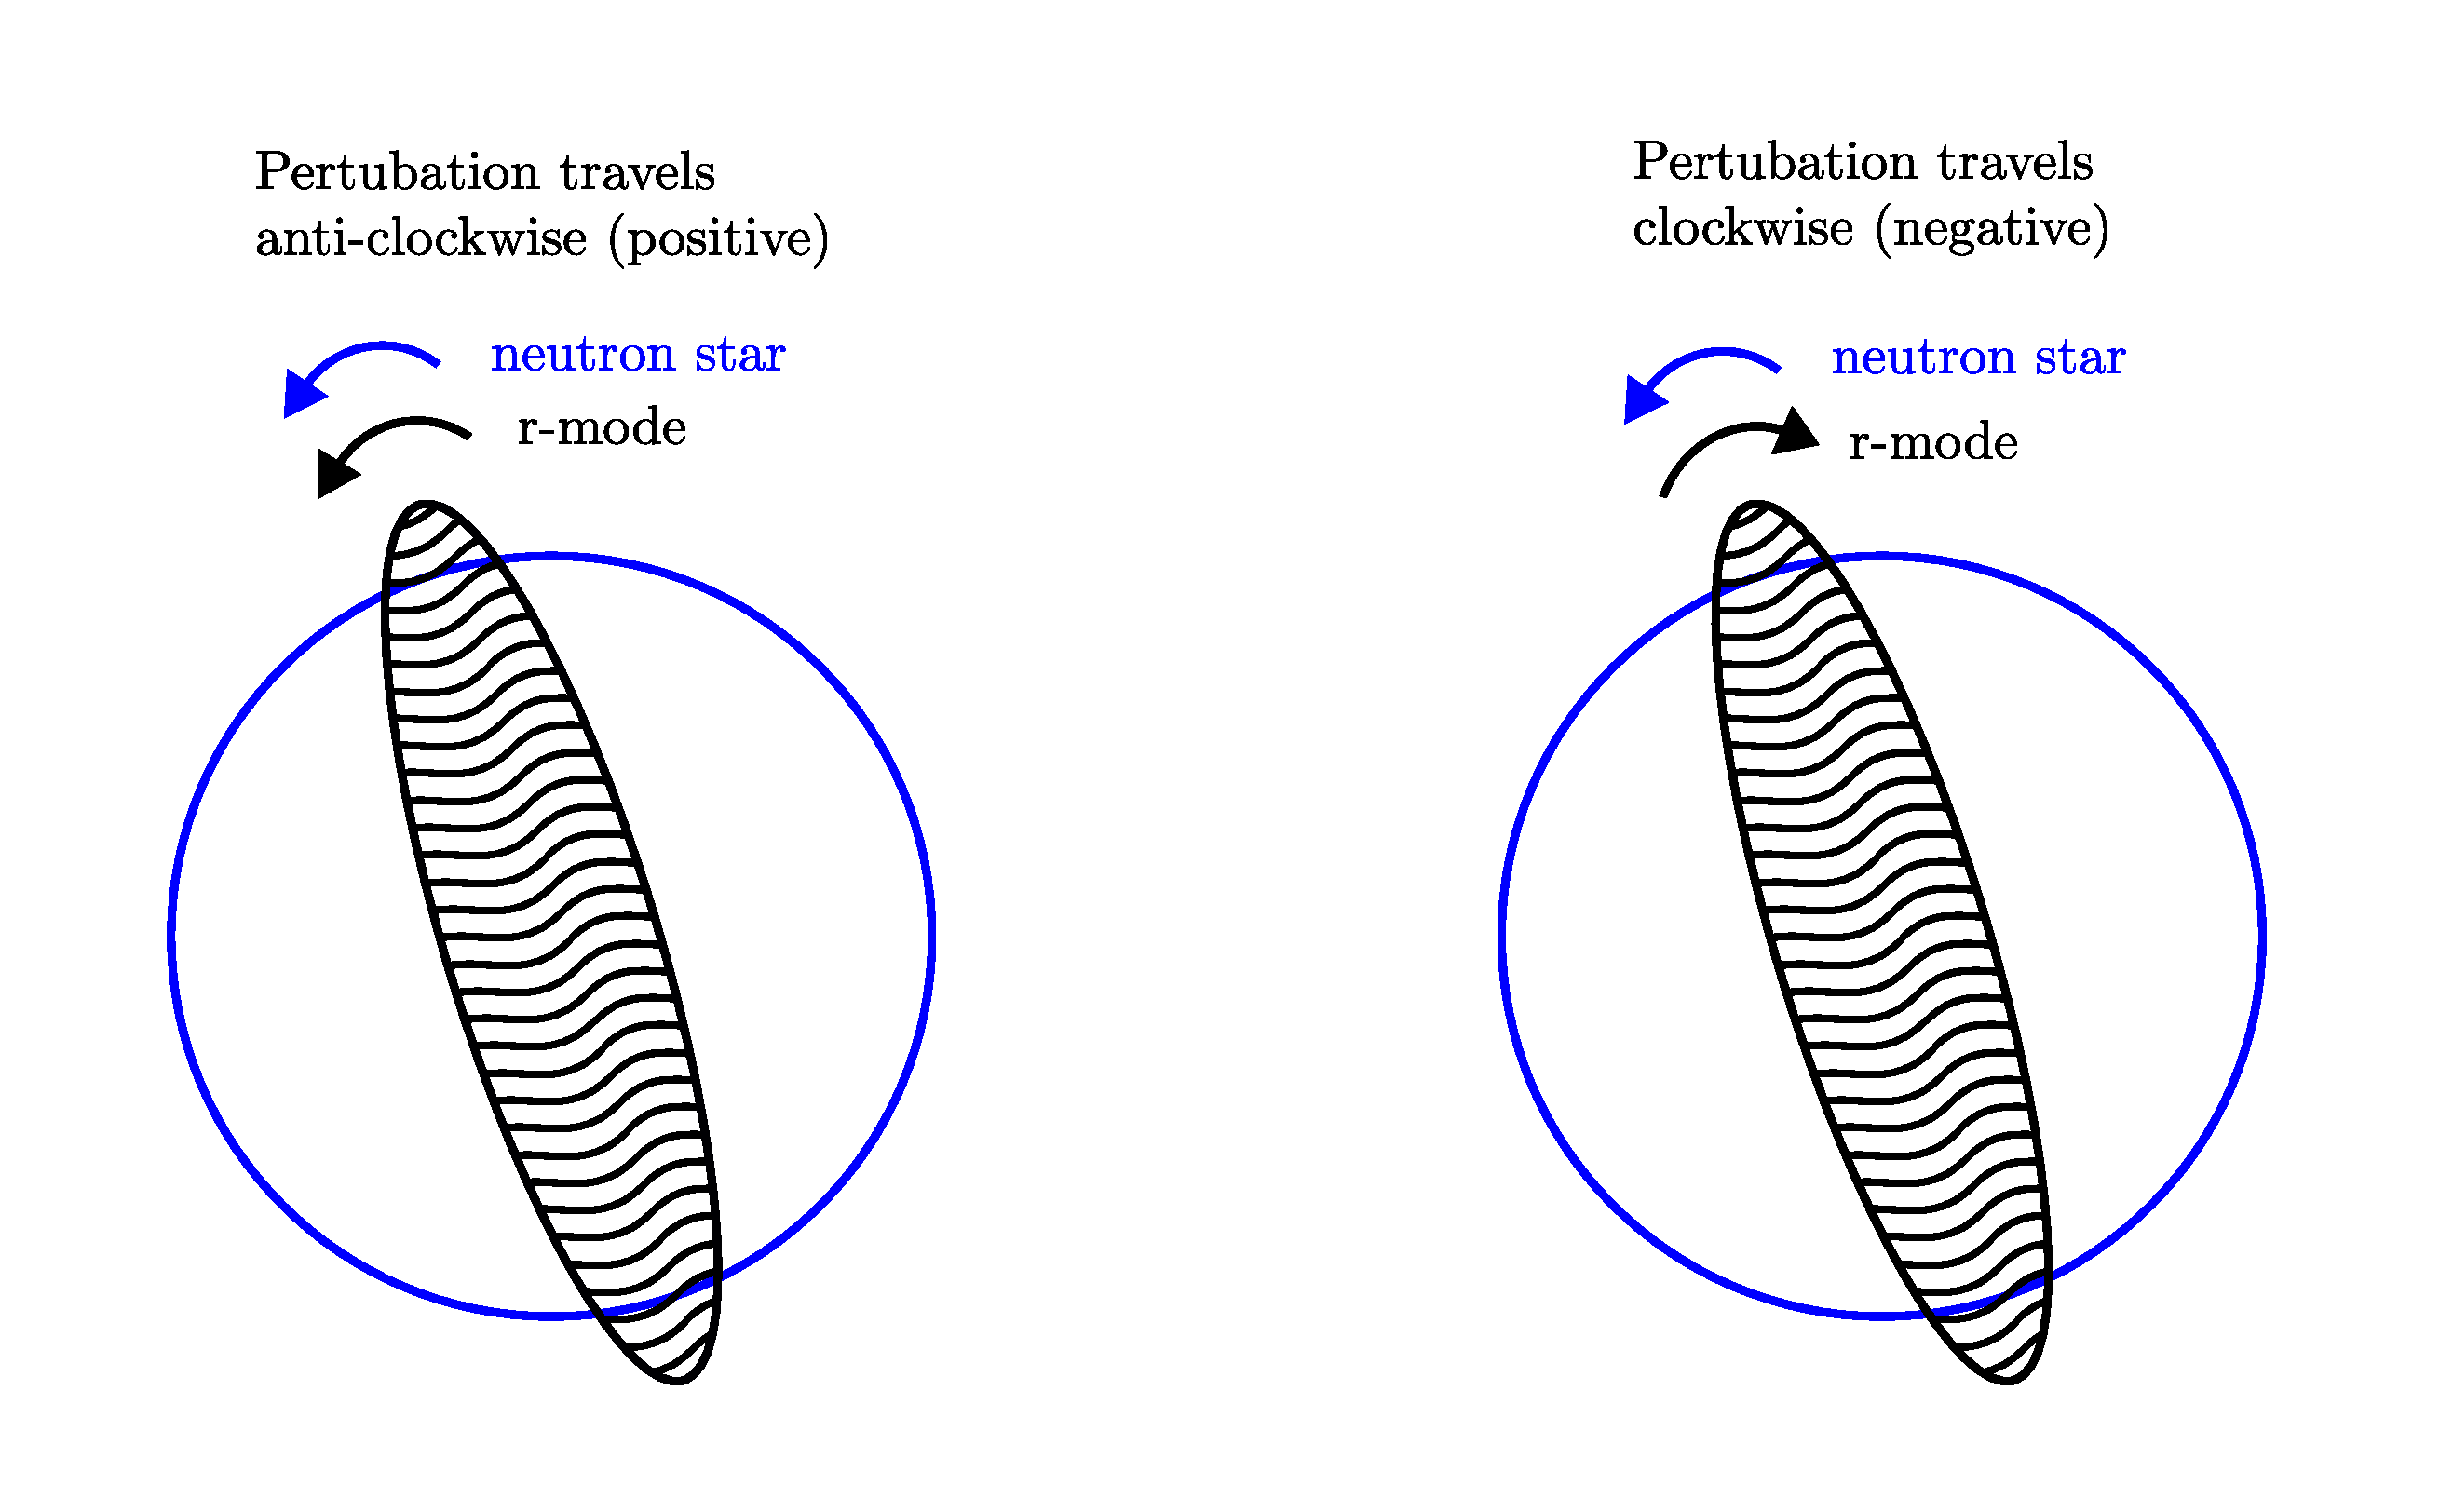
\includegraphics[width=\textwidth]{C1_intro/rmode.pdf}
	\caption[Generating \glspl{GW} from r-modes in neutron stars.]{The r-modes can travel in either direction in the star. in the case when the r-mode is moving clockwise and the neutron star is moving anti-clockwise, if the neutron star is rotating fast enough it can cause unstable emission of \gls{GW}. This image was reconstructed from \citep{jonesCFSInstability}.}
	\label{intro:source:cw:rmode}
\end{figure}
If these modes are excited in a non-rotating star, then they will emit \gls{GW} where the \gls{GW}  carries away angular momentum \citep{jonesCFSInstability}. 
For the mode travelling in a clockwise direction, this angular momentum is positive and the mode travelling anti-clockwise the angular momentum is negative. 
Therefore, the \gls{GW} is taking away either positive or negative angular momentum (adding angular momentum) depending on the direction of rotation.
The emission of \gls{GW} damps the modes and the magnitude of the perturbation decreases making them extremely difficult to detect.
Now if the neutron star is rotating, this can lead to an effect called the \gls{CFS} instability  \citep{chandrasekhar1970SolutionsTwo,friedman1978SecularInstability}. 
As the rotation speed of the neutron star increases, there are two different effects on the modes travelling in opposite directions. 
For the mode travelling anti-clockwise with the stars rotation, the mode will appear to be travelling faster, therefore, will emit more \gls{GW} taking away more angular momentum. This means that this mode will be damped more rapidly.
The interesting affect is for the mode travelling clockwise, opposite to the neutron stars rotation. 
At a certain rotation rate, the mode will be `frozen' from the observers perspective and no \gls{GW} will be emitted.
As the rotation rate increases further, the mode will appear to travel anti-clockwise to an observer, i.e. the mode is dragged in the opposite direction by the stars rotation. 
Here it is key to remember that this mode had negative angular momentum as in the neutron stars frame it is still travelling clockwise.
As the mode rotates its emits positive angular momentum, which is then subtracted from the modes negative angular momentum.
The magnitude of the angular momentum then increases such that more \glspl{GW} are released.
This effect causes the amplitude of the oscillation to grow and therefore become unstable.
Therefore, a neutron star is unstable to \gls{GW} emission if it is rotating sufficiently fast \citep{lasky2015GravitationalWaves}.
For a more detailed view on how r-modes generate \gls{GW} see \citep{owen1998GravitationalWaves,jonesCFSInstability}


%%%%%%%%%%%%%%%
%%%%%%%%%%%%%%
%%%%%%%%%%%%%%%
\section{\label{intro:detector}Detectors}
%%%%%%%%%%%%%%%%
%%%%%%%%%%%%%%
%%%%%%%%%%%%%%

The indirect detection of gravitational waves from the Hulse-Taylor binary pulsar system left little doubt that \gls{GW} existed. 
The real challenge was to design an instrument which could directly detect gravitational waves.
There were a number of different proposed methods for the design of the instrument, notably: resonant bar detectors, both ground based and space based interferometers, pulsar timing arrays and cosmic microwave background (CMB) detectors. 
The first resonant bar detector was designed and built by Joseph Weber \citep{weber1966ObservationThermal}. 
These are large cylinders of metal which should resonate as a gravitational wave passes by. 
There are a few different designs of this type of detector, including an omni-directional design \citep{dewaard2003MiniGRAILFirst}. 
Pulsar timing arrays aim to use the accurate arrival time of pulses from millisecond pulsars to measure \gls{GW} \citep{hobbs2017GravitationalWave}. As a \gls{GW} passes between the pulsar and the observer, the arrival time of the pulses should change by $\mathcal{O}(10)$ ns \citep{hobbs2017GravitationalWave}. 
Whilst a detection has not been made using pulsar timing arrays, these methods are still in use.
Cosmic microwave background detectors aimed to look for evidence of gravitational waves in the polarisation's of the CMB \citep{ade2018ConstraintsPrimordial}.  
These use the a range of detectors to look at the CMB however, are yet to confirm a detection of a \gls{GW} signal.
The most commonly known design of a \gls{GW} detector is the ground based interferometer, these made the first detection of \gls{GW} in 2015 \citep{abbott2016ObservationGravitational}. 
These are the focus of this section as the analysis that will follow uses data from the \gls{LIGO} detectors in the USA \citep{abbott2009LIGOLaser,aasi2015AdvancedLIGO} and Virgo detector in Italy \citep{acernese2015AdvancedVirgo,acernese2008StatusVirgo}. 

%%%%%%%%
%%%%%%%%%
\subsection{Laser Interferometers}
%%%%%%%%%%
%%%%%%%%%

Laser interferometers use the interference of light to measure a length with high precision.
The majority of this section will focus on ground based interferometers such as \gls{LIGO} and Virgo \citep{aasi2015AdvancedLIGO,acernese2015AdvancedVirgo}.
A simple design of an interferometer is shown in Fig.~\ref{detectors:interferometer:simple}. 
A laser beam is fired at a beam splitter which splits the light equally down two perpendicular arms. 
Each of these beams is reflected from a mirror at the end of either arm.
The light then returns to the beam splitter where the two beams are combined and sent to a photo-detector.
At the output, there is an interference pattern between the two beams.
If the length of one of the arms is changed then the interference pattern will change as the phase of one beam changes with respect to the other.
The phase difference of the light can be related to the wavelength of the light, $\lambda_l$ and the length of the detectors arms $L$ by
\begin{equation}
\label{intro:detectors:phasechange}
\Delta \phi \sim \frac{\Delta L}{\lambda_l},
\end{equation}
where $\Delta  \phi$ is the phase change and $\Delta L$ is the difference in the arm lengths.
An interferometer can then measure small changes in the mirrors position.
\begin{figure}[hp]
    \centering
    \begin{subfigure}[h]{0.6\linewidth}
    	 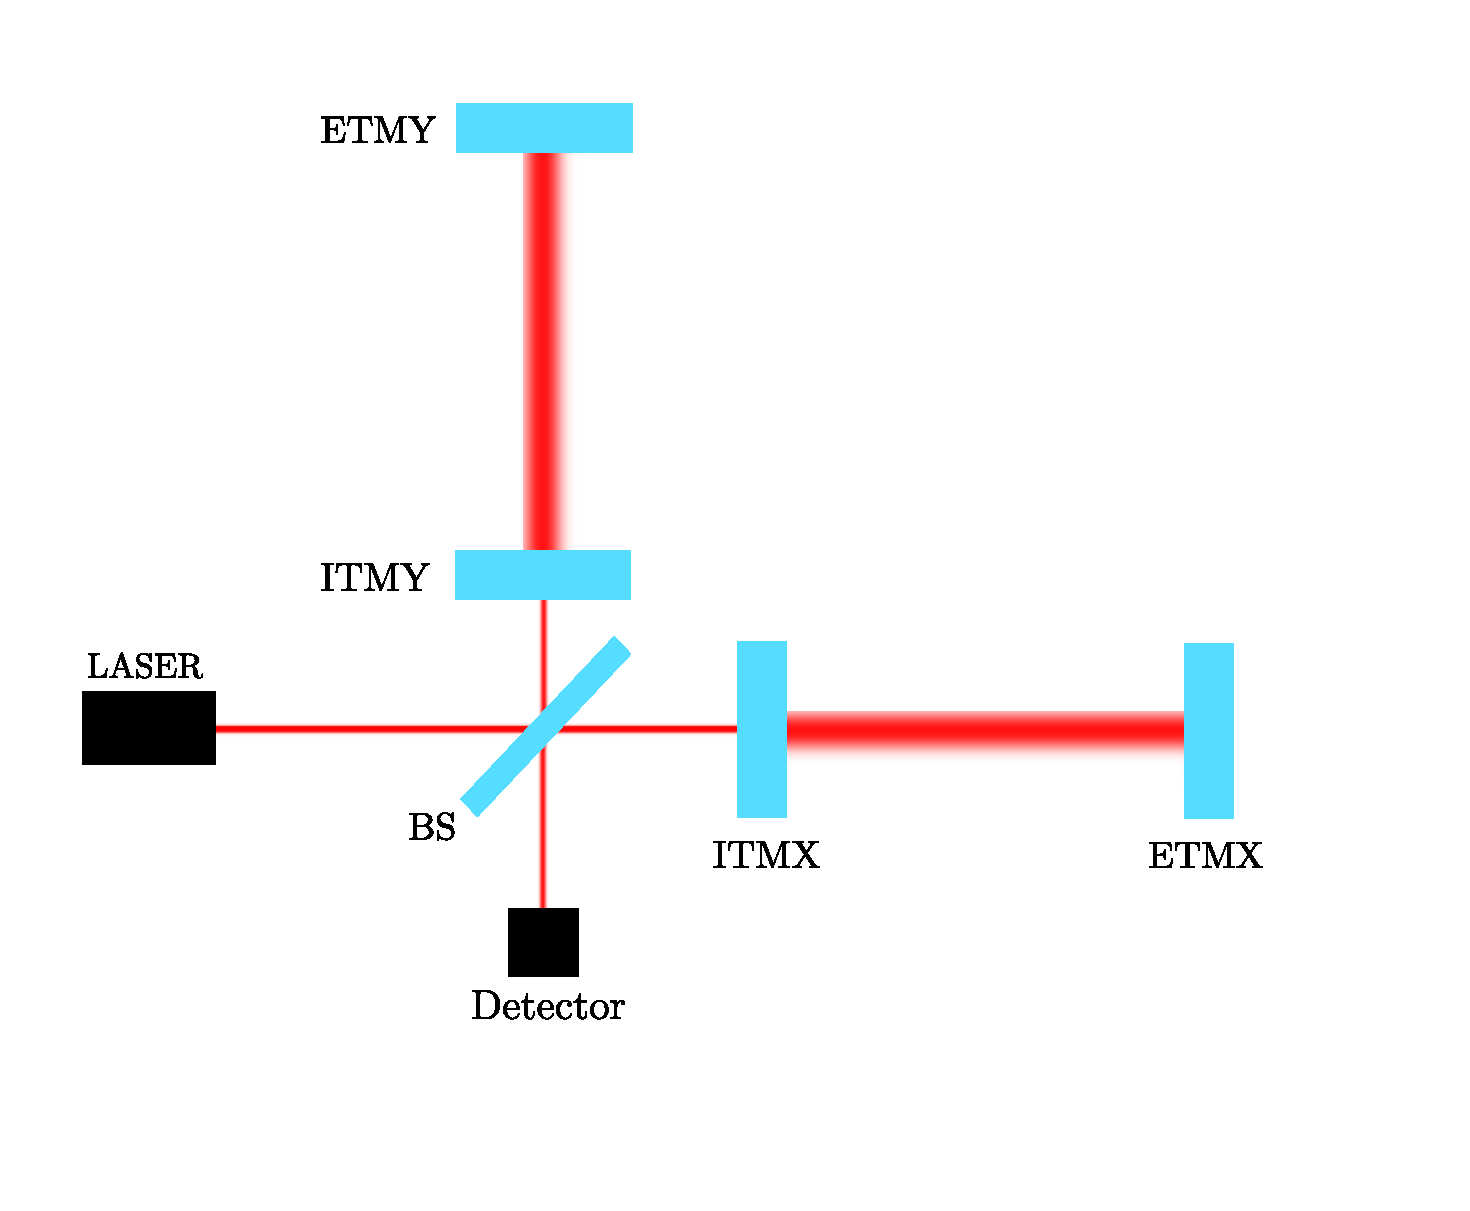
\includegraphics[width=\textwidth]{C1_intro/interferometer.pdf}
    	 \caption{Simple interferometer.}
    	 \label{detectors:interferometer:simple}
    \end{subfigure}
	\begin{subfigure}[h]{0.6\linewidth}
		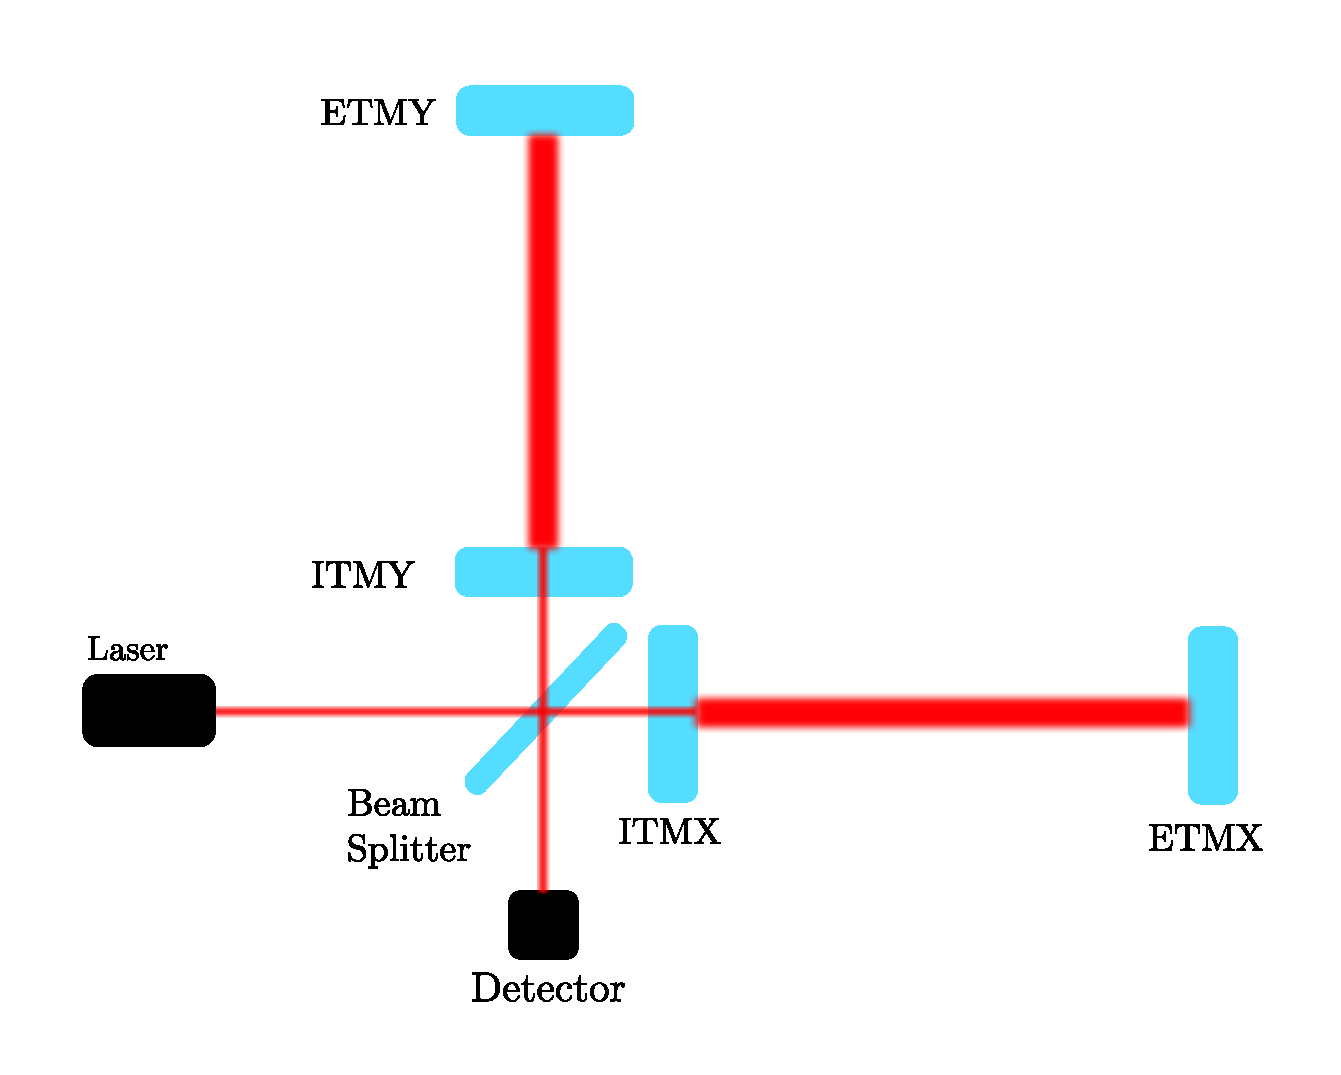
\includegraphics[width=\textwidth]{C1_intro/interferometer_fabry.pdf}
		\caption{Fabry-Perot interferometer.}
		\label{detectors:interferometer:fabry}
	\end{subfigure}
    \caption[Basic layout of the \gls{LIGO} detectors.]{\gls{LIGO} uses interferometry to make a detection. This has many additional features, one of which is shown above. ETMY and ETMX refer to the end test masses, which are just mirrors at the end of the interferometer arms. The beam splitter splits the Laser beam equally to each arm, this them recombines the beams back to the detector.
    ITMY and ITMX refer to the internal test masses, these create a Fabry-Perot cavity in the interferometers arms which can build up laser power. }
    \label{detectors:interferometer}
\end{figure}
%
This can be used in gravitational wave detection as the mirrors at the end of each arm of the interferometer can be treated as `free' test masses.
Figure \ref{gw:polarisations} shows the effect of a \gls{GW} on free test masses.
One can see this by looking at the proper separation between two test masses. 
If we place two test masses along the $x$ axis with separation $L_c$ where a gravitational wave is travelling along the $z$ axis, the proper distance between them is given by
\begin{equation}
    L = \int_{0}^{L_c} \sqrt{g_{xx}} dx,
\end{equation}
where $g_{xx} = 1 + h_{+}(t)$ is the combination of Eq.~\ref{intro:gravwave:metric} and Eq.~\ref{intro:gw:gravwave}. 
As the metric perturbation is small is can be can be expanded to first order, i.e. $\sqrt{g_{xx}} = \sqrt{1 + h_{+}(t)} \approx 1 + \frac{1}{2}h_{+}(t)$.
The proper distance is then
\begin{equation}
    \label{intro:detectors:properdist}
    \begin{split}
     L &\approx \int_{0}^{L_c} 1 + \frac{1}{2}h_{+}(t) dx \\
      &\approx L_c + L_c \frac{1}{2}h_{+}(t).
    \end{split}
\end{equation}
From Eq.~\ref{intro:detectors:properdist} on can see that in this configuration the plus polarisation of the gravitational wave causes the separation between the two test masses to oscillate \citep{flanagan2005BasicsGravitational}.
This can then be oscillation can be expressed as a fractional length change 
\begin{equation}
    \label{intro:detectors:fraclength}
    \frac{\delta L}{L} \approx \frac{1}{2} h_{+}.
\end{equation}
In the interferometer, this affect changes the lengths of the two arms which therefore changes $\Delta L$ in Eq.~\ref{intro:detectors:phasechange}.
The change of the interference pattern with time is then related to the \gls{GW}.
In practice the position of the two mirrors are held in position such that the interference pattern does not change.
The \gls{GW} is then related to the readout of the mirrors control system.

If one looks at Eq.~\ref{intro:detectors:fraclength} then if the mirrors at the end of the arms (ETMX and ETMY) are are placed further from the beam splitter, i.e. $L$ is increased, then the length change of the arms due to the gravitational wave will be greater.  
This means that increasing the length of the detectors arms increases the sensitivity of the interferometer. 
A method to achieve a similar affect without physically increasing the arm length is to use a Fabry-Perot cavity \citep{aasi2015AdvancedLIGO}, this is shown in Fig.~\ref{detectors:interferometer:fabry}.
This is where a semi-transparent mirror is placed between the beam splitter and end mirror in each arm (ITMX and ITMY).
Light enters this cavity and reflects back and forth between the two mirrors (ITMX and ETMX) a number of times before returning to the beam splitter.
This increases the time the light spends in one arm and is equivalent to increasing the arm length.
Actual ground based \gls{GW} detectors such as \gls{LIGO} \citep{abbott2009LIGOLaser} and Virgo \citep{acernese2015AdvancedVirgo} are much more complicated than described above.
They use many techniques to increase the sensitivity some of which are outlined in \citep{aasi2015AdvancedLIGO,abbott2009LIGOLaser}.
Many of these techniques are designed to reduce non-astrophysical affects on the detector, some of these effects and solutions are listed in Sec.~\ref{intro:detector:noise}.



%%%%%%%%%%%
%%%%%%%%%%
\subsubsection{Detector response}
%%%%%%%%%%
%%%%%%%%%

An important factor to know when using detector data to search for astrophysical signals is the detectors antenna pattern.
This measures how sensitive the detector is to different directions.
An example of the antenna response for \gls{LIGO} is in Fig.~\ref{intro:detectors:response} where the detectors arms lie on the x and y axis of the image.
This is clear when thinking about how a gravitational wave affects the test masses as in Fig.~\ref{gw:polarisations}. 
As the \gls{GW} is transverse to its propagation, when the detector is face on to the source, there will be a maximum change in the arm lengths and therefore a maximum sensitivity. 
In the same way the sensitivity will be at a minimum when edge to the source.

\begin{figure}
    \centering
    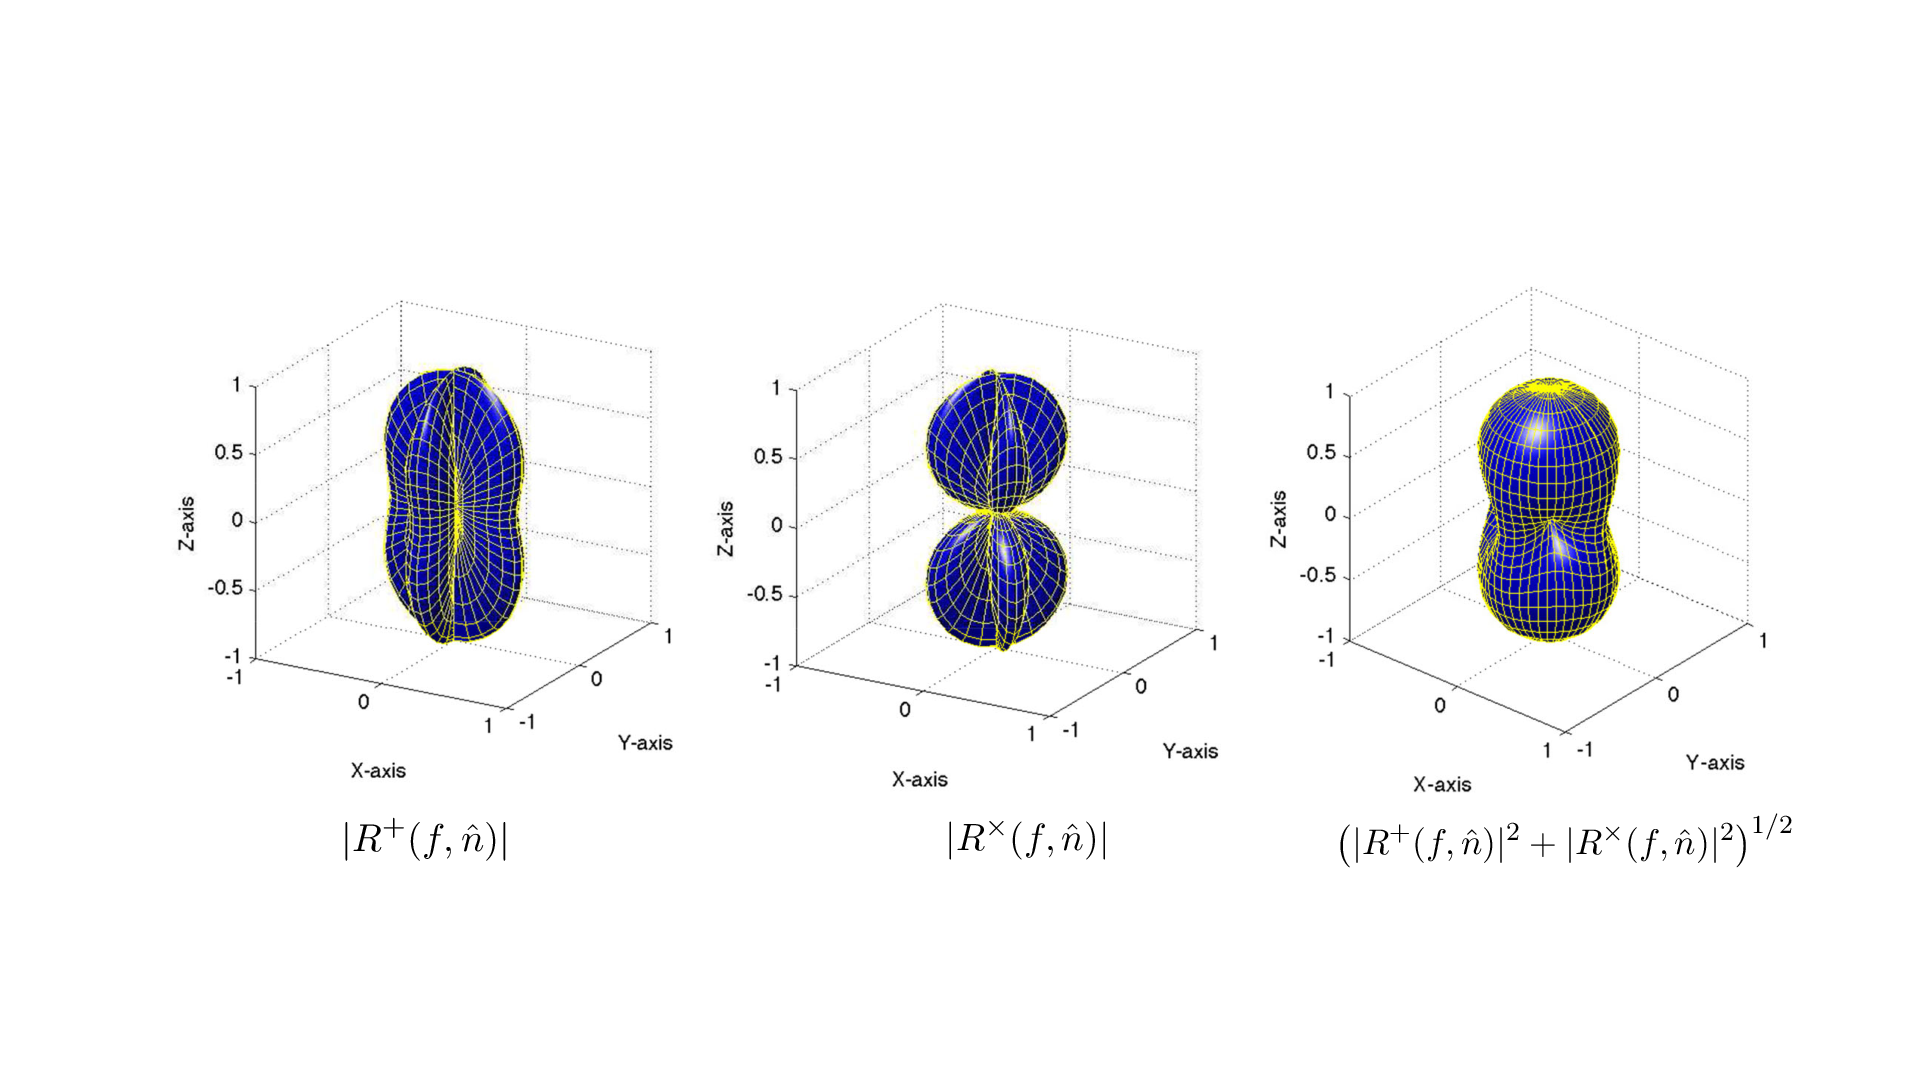
\includegraphics[width=\textwidth]{C1_intro/LIGO_beam_patterns.png}
    \caption[Antenna response of the \gls{LIGO} detectors.]{The antenna response is shown as in \citep{romano2019SearchesStochastic} for both the plus and cross polarisations and their average. The detectors arms lie on the x and y axis in the above plots. }
    \label{intro:detectors:response}
\end{figure}

%%%%%%%%%%%
%%%%%%%%%%
\subsubsection{\label{intro:detector:noise}Noise sources}
%%%%%%%%%%
%%%%%%%%%%

To increase the sensitivity of the \gls{LIGO} detectors, any effect on the output of the interferometer which is not astrophysical ideally needs to be reduced.
This involves understanding what causes certain noise features in the detector, and how the affect of these can be limited. 
Within the detector, there are many sources of noise.
Some of these noise sources and how they limit the detectors strain sensitivity are all shown in Fig.~\ref{detectors:noisesensitivity} from \citep{aasi2015AdvancedLIGO}.
\begin{figure}[h]
    \centering
    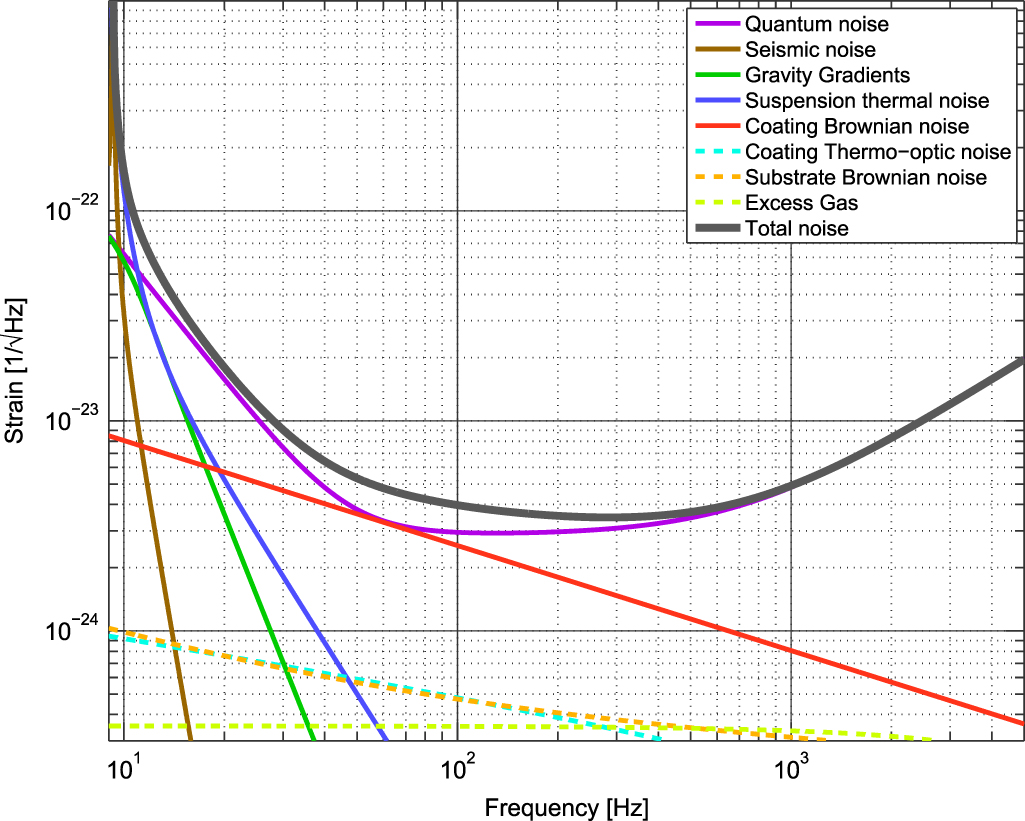
\includegraphics[width=0.9\textwidth]{C1_intro/noise_sensitivity.jpg}
    \caption[Example strain sensitivity curves for different noise sources in \gls{LIGO}.]{The different noise sources affect the sensitivity of the \gls{LIGO} detectors at different frequencies. This shows the various sources how the affect the noise curve \citep{aasi2015AdvancedLIGO}.}
    \label{detectors:noisesensitivity}
\end{figure}
Here I will summarise some of the limiting sources and also sources which become useful for understanding later sections.

\begin{description}
\item[Seismic noise] This originates from vibrations in the earth which can be from effects such as the earths seismic activity or anthropogenic sources. This affects lower lower frequencies of \glspl{LIGO} spectrum. This can be oscillations such as earthquakes or ocean waves. Seismic waves cause the mirrors to oscillate and induce a change in the length of the arm. This is reduced by having multi stage suspensions in the detectors which filter out the seismic oscillations \citep{matichard2015SeismicIsolation}.

\item[Coating noise] This is in general due to two main factors, the thermal noise of the coating and Brownian noise. The Brownian noise is from the mechanical dissipation in the coating and the thermal noise is due to thermal dissipation. The Brownian noise is the dominant factor as shown in Fig.~\ref{detectors:noisesensitivity}. These effects are limited by using different coatings on the mirrors \citep{abernathy0OverviewResearch}.

\item[Quantum noise] Quantum noise is a fundamental limit due to the statistical uncertainty of counting photons. This limits the sensitivity at many frequencies.There are methods to reduce this include squeezing of the light \citep{aasi2013EnhancedSensitivity}. 

\item[Electronics noise \joe{technical noise maybe}] Whilst this is not shown in Fig.~\ref{detectors:noisesensitivity}, this becomes important to searches described later. These have a different effect on the detector which is more narrowband frequency lines. This is generated by the digital and analogue electronics that are used to measure the signal. 
\end{description}

There are also many other sources of noise in the detector which I have not listed. However, these are often not the limiting cases of noise or are not relevant to this thesis.
In Sec.~\ref{detchar} I will go into more detail about specific noise sources in the detector known as instrumental lines and how they can be monitored and potentially removed. 













% and the other chapters

\chapter{SOAP Search}


\section{Viterbi algorithm}
%
% Into to viterbi
%
The Viterbi algorithm is an efficient method for determining the most probable set of states (a single `track' of steps on the time-frequency plane) in a Markov model dependent on data, where the model has a discrete number of states at each step. Rather than computing the probability of every possible track and selecting the most probable, the algorithm maximises this probability after every discrete step. As a result, a partial track which cannot ultimately be the most probable is rejected before the next step is calculated, and only a fraction of all possible tracks need to be computed to find the one that is most probable.

%
% Defining varibles and what data we use
%
In this work we apply the Viterbi algorithm to a \ac{GW} strain time-series to find the most probable track of a single variable-frequency signal in the noisy data.  We divide the time series into $N$ equal-length and contiguous segments ${\bm x}_j$,  defining the set $D \equiv \{{\bm x}_j\}$. The `states' in the model correspond to the frequencies a signal could have in each segment. A `track' is a list of such frequencies ${\bm \nu}\equiv \{\nu_j\}$, where  $\nu_j$ is the frequency in the segment ${\bm x_j}$.

%
% defining probabilities
%
Our objective is to calculate the most probable track given the data, i.e., the
track that maximises $p({\bm \nu}\mid D)$. Using Bayes theorem, this posterior probability can
be written as
%
\begin{equation}
\label{viterbi:bayes}
  p({\bm \nu} \mid D) = \frac{p({\bm \nu})p(D \mid {\bm \nu})}{p(D)},
\end{equation}
%
where $p({\bm \nu}) $ is the prior probability of the
track, $p(D \mid{\bm \nu})$ is the likelihood of the track (i.e., the
probability of the data given the track) and $p(D)$ is the model evidence (or
marginalised likelihood).

The Viterbi algorithm treats the track as the result of a Markovian process,
such that the current state depends only on the previous state. It is
therefore useful to split the track's prior into a set of transition
probabilities such that
%
\begin{align}
\label{viterbi:prior}
p({\bm \nu}) &= p(\nu_{N - 1}, \ldots, \nu_1, \nu_0)\nonumber \\
%&=  p(\omega_{N} \mid \omega_{N-1}, \ldots, \omega_1,\omega_0)p(\omega_{N-1} \mid \omega_{N-2}, \ldots, \omega_1,\omega_0) \ldots p(\omega_1 \mid \omega_0)p(\omega_0) \\
&= p(\nu_{N - 1} \mid \nu_{N-2})p(\nu_{N-2} \mid \nu_{N-3}) \dots p(\nu_1 \mid \nu_0)p(\nu_0) \nonumber \\
&= p(\nu_0)\prod_{j=1}^{N-1}p(\nu_{j} \mid \nu_{j-1}),
\end{align}
%
where $p(\nu_0)$ is the prior probability that the signal in the first time
step has a frequency $\nu_0$ and $p(\nu_{j} \mid \nu_{j-1})$ is the
prior `transition' probability for $\nu_j$ given the frequency at the last
step was $\nu_{j-1}$.

The noise in each of the segments can be treated as independent, so the
likelihood component in Eq.~\ref{viterbi:bayes} can be factorised as
%
\begin{equation}
\label{viterbi:likelihood}
p(D \mid {\bm \nu}) = \prod_{j=0}^{N-1}p({\bm x_j} \mid \nu_j),
\end{equation}
%
 where $p({\bm x_j} \mid \nu_j)$ is the likelihood of our
signal having a frequency $\nu_j$ in the $j$th segment.

Using Eqs.~\ref{viterbi:bayes},\ref{viterbi:prior} and
\ref{viterbi:likelihood}, the posterior probability is then
%
\begin{equation}
\label{viterbi:posterior}
    p({\bm \nu} | D) =
    \frac{p(\nu_0)p({\bm x_0} | \nu_0) \displaystyle\prod_{j=1}^{N-1}p(\nu_{j}
| \nu_{j-1})p({\bm x_j} | \nu_j)}{\displaystyle\sum_{S}
\left\{p(\nu_0)p({\bm x_0} | \nu_0)\displaystyle\prod_{j=1}^{N-1}p(\nu_{j} |
\nu_{j-1})p({\bm x_j} | \nu_j)\right\}} ,
\end{equation}
%
where in the denominator we must sum over all possible tracks
$S$~\cite{Slade2014}. We require the specific track, or set of frequencies, $\hat{\bm
\nu}$ that  maximises the posterior probability, and which therefore
maximises the numerator  on the right-hand side of  Eq.~\ref{viterbi:posterior}, i.e.,
%
\begin{equation}
\label{viterbi:maxtrack}
  p(\hat{\bm \nu} | D) \propto \max_{\bm \nu}{\left[p(\nu_0)p({\bm x_0} |
\nu_0) \prod_{j=1}^{N-1}p(\nu_{j} |\nu_{j-1})p({\bm x_j} | \nu_j)\right]}.
\end{equation}
%
This track also maximises the log of the probability,
%
\begin{equation}
\label{viterbi:maxtracklog}
\begin{split}
  \log p(\hat{\bm \nu} | D)  = \max_{{\bm \nu}}{\biggl\{ \log p(\nu_0) + \log p({\bm x_0} | \nu_0)  } \\
 \left. \sum_{j=1}^{N-1} \biggl[ \log p(\nu_{j} | \nu_{j-1}) + \log p({\bm x_j}
| \nu_j) \biggr] \right\} + \text{const}.
  \end{split}
\end{equation}
%
The Viterbi algorithm finds the most probable track $\hat{\bm \nu}$ by calculating the quantities in Eq,~\ref{viterbi:maxtracklog} for each frequency at each time step. In the following sections we explain how this is achieved in practice.

%%%%%%%%%%%%%%%%%%%%%%%%%%%%%%%%%%%%%%%%%%%%%%%%%%%%%%%%%%%%%%%%%%%%%%%%%
%%%%%%%%%%%%%%%%%%%%%%%%%%%%%%%%%%%%%%%%%%%%%%%%%%%%%%%%%%%%%%%%%%%%%%%%%
\section{\label{viterbi:transition}The transition matrix}
%%%%%%%%%%%%%%%%%%%%%%%%%%%%%%%%%%%%%%%%%%%%%%%%%%%%%%%%%%%%%%%%%%%%%%%%%
%
% define the transition matrix
%
We define the `transition matrix' $T$ as the matrix that stores the prior log-probabilities $\log p(\nu_j \mid \nu_{j-1})$. These transition probabilities depend only on the size and direction of the transition, and in our case correspond to a jump in frequency when moving from the $(j-1)$th to the $j$th state. It is within the transition matrix that we impose some loose model constraints. For example it is usual in the time-frequency plane for frequencies to only have discrete values (frequency bins) and a track might only be allowed to move by one bin in each time step, restricting it to a \ac{UCD} transition or `jump' or equivalently setting the size of the first dimension of the transition matrix $n_1 = 3$. We can also impose that the transition probabilities are independent of the current track location in frequency, i.e. $p(\nu_j \mid \nu_{j-1})=p(\nu_{j+k} \mid \nu_{j+k-1})$. This leads to the transition matrix containing only three numbers, corresponding to the three prior log-probabilities that the track was in the corresponding \ac{UCD} frequency bin at the previous time step. These numbers are chosen to reflect the prior probability of a frequency deviation in the track and depend on the class of signals that one wishes to detect.

In later sections we will consider more complex situations in which the transition matrix describes the prior probability associated with sequences of even earlier transitions (`memory') and the case where there are multiple detectors. In these cases the number of dimensions of the transition matrix can grow substantially to account for the extra complexity of the problem.

%%%%%%%%%%%%%%%%%%%%%%%%%%%%%%%%%%%%%%%%%%%%%%%%%%%%%%%%%%%%%%%%%%%%%%%%%
%%%%%%%%%%%%%%%%%%%%%%%%%%%%%%%%%%%%%%%%%%%%%%%%%%%%%%%%%%%%%%%%%%%%%%%%%
\section{\label{viterbi:single}Single detector}
%%%%%%%%%%%%%%%%%%%%%%%%%%%%%%%%%%%%%%%%%%%%%%%%%%%%%%%%%%%%%%%%%%%%%%%%%
%
% single detector algorithm,
%
We will first consider the simple case of a single dataset $D$, generated by a single gravitational wave detector, and consider only a one-dimensional transition matrix. We will make use of discrete Fourier transforms so that frequencies, and hence the track frequencies, are also discrete. These frequencies will be indexed by $k$ and therefore $\nu_j \rightarrow \nu_{j,k}=k(j)\Delta f$ where $\Delta f=1/T$ is the frequency bin width for a segment of duration $T$.

 The Viterbi algorithm determines the most probable track on the time-frequency plane by calculating the value of Eq.~\ref{viterbi:maxtracklog} for every discrete Fourier frequency, incrementally in time. In other words, at each time segment it finds the most probable earlier track which ends at each particular frequency. On reaching the final segment it can look back to identify the most probable track connecting segment 1 to segment $N$.

There are two main components to Eq.~\ref{viterbi:maxtracklog}: the transition probabilities $p(\nu_j \mid \nu_{j-1})$ and the likelihoods $p({\bm x_j} \mid \nu_j)$. The transition probabilities are pre-calculated and stored in a transition matrix according to Sec.~\ref{viterbi:transition} above, and details of how these are calcuated are described in Sec.~\ref{results}. To calculate the likelihood we follow the approach of~\cite{Bretthorst1988} which gives, under the assumption of a single sinusoidal signal in additive Gaussian noise in data segment ${\bm x_j}$,
%
\begin{equation}
\label{viterbi:single:likelihood}
p({\bm x_j} \mid \nu_{j,k}, \sigma_{j,k}, I) \propto
\exp\left[{C(\nu_{j,k})}\right].
\end{equation}
%
where
$C_{j,k}(\nu_{j,k})$ is the Schuster periodogram normalised to the noise variance at
frequency $\nu_{j,k}$ of segment $j$. This is equivalent to the log-likelihood, and is defined as
%
\begin{equation}
\label{viterbi:periodogram}
C(\nu_{j,k}) \equiv C_{j,k}=  \frac{1}{\sigma_{j,k}^2}\frac{1}{N_{\rm s}}\left|\sum_{r=0}^{N_{\rm
s}-1}x_{j,r} {\rm
e}^{i\nu_{j,k} t_r}\right|^2,
\end{equation}
%
where $N_{\rm s}$ is the number of data points in each segment and $t_{r}$ is the time corresponding to $x_{j,r}$, the $r$th sample in the $j$th data segment. $\sigma_{j,k}^2$ is the noise variance and is calculated as an estimate of the noise \ac{PSD} in the $k$th sample and the $j$th data segment. It is worth noting at this point that it is also possible to write this as a likelihood ratio, and therefore write out detection statistic as a log-odds ratio, however, we will discuss this in more depth in Sec.~\ref{viterbi:las}. The log-likelihoods of each segment can be calculated at discrete frequencies before running the algorithm by computing the power spectra for each segment from discrete Fourier transforms of the data. In the \ac{GW} field these standard data forms are known as \acp{SFT}.

The Viterbi algorithm records two quantities for each frequency and time bin: The first, $V_{j,k}$, contains the value defined by Eq.~\ref{viterbi:maxtracklog}, which is the log-probability of the most probable path ending in position $j,k$. The second, $A_{j,k}$, is the transition, or `jump', used to achieve the most probable path. The algorithm can be divided into three main sections: initialisation, iteration and identification. These three sections are described in pseudo-code in Alg.~\ref{viterbi:single:algorithm} and a simple demonstration of the algorithm at work is shown in Fig.~\ref{viterbi:plots}.
%
%
%   pseudo algorithm
%
\begin{algorithm}
\begin{algorithmic}[1]
\STATE{Input: ${C}$, $T$} \COMMENT{log-likelihood,transition matrix}
\STATE{Output: $\hat{\bm \nu}$, $V$, $A$} \COMMENT{most probable track, track probabilities, jumps}
\STATE
\STATE{ {\it Initialisation}}
\FOR{Frequency ($\nu_{0,k}$), $k=0 \rightarrow M-1$}
    \STATE{$V_{0,k} =  { C_{0k}} $ }
    \STATE{$A_{0,k} = 0$}
\ENDFOR
\STATE
\STATE{ {\it Iteration}}
\FOR{Segment, $j=0 \rightarrow N-1$}
    \FOR{Frequency ($\nu_{j,k}$), $k=0 \rightarrow M-1$}
        \STATE{$V_{j,k} = {\max\limits_{i }  ({ C_{j,k}} + T_i + V_{j-1,j+i})}$}
        \STATE{$A_{j,k} = {\argmax\limits_{ i }  ({ C_{j,k}} + T_i + V_{j-1,j+i})}$}
    \ENDFOR
\ENDFOR
\STATE
\STATE{ {\it Identification}}
\STATE{$\hat{\nu}_{N-1} = \argmax_k (V_{N-1,k})$}
\FOR{Segment, $j=N-1 \rightarrow 0$}
	\STATE{$\hat{\nu}_j = \hat{\nu}_{j+1} + A_{j,\nu_{k+1}}$}
\ENDFOR
%
\end{algorithmic}
\caption{The Viterbi algorithm in pseudo-code. $N$ is the number of segments, $M$ is the number of frequency bins in each segment. Here the maximisations over $i$ run between $\pm (n_1-1)/2$ where $n_1$ is the size of the transition matrix. The values from Eq.~\ref{viterbi:maxtracklog} are stored in $V$, and the jumps are stored in $A$. The most probable track is denoted by $\hat{\bm \nu}$.\label{viterbi:single:algorithm}}
\end{algorithm}
%
%
% example plot to work through
%
%
\begin{figure}
\centering
\begin{subfigure}[h]{0.8\columnwidth}
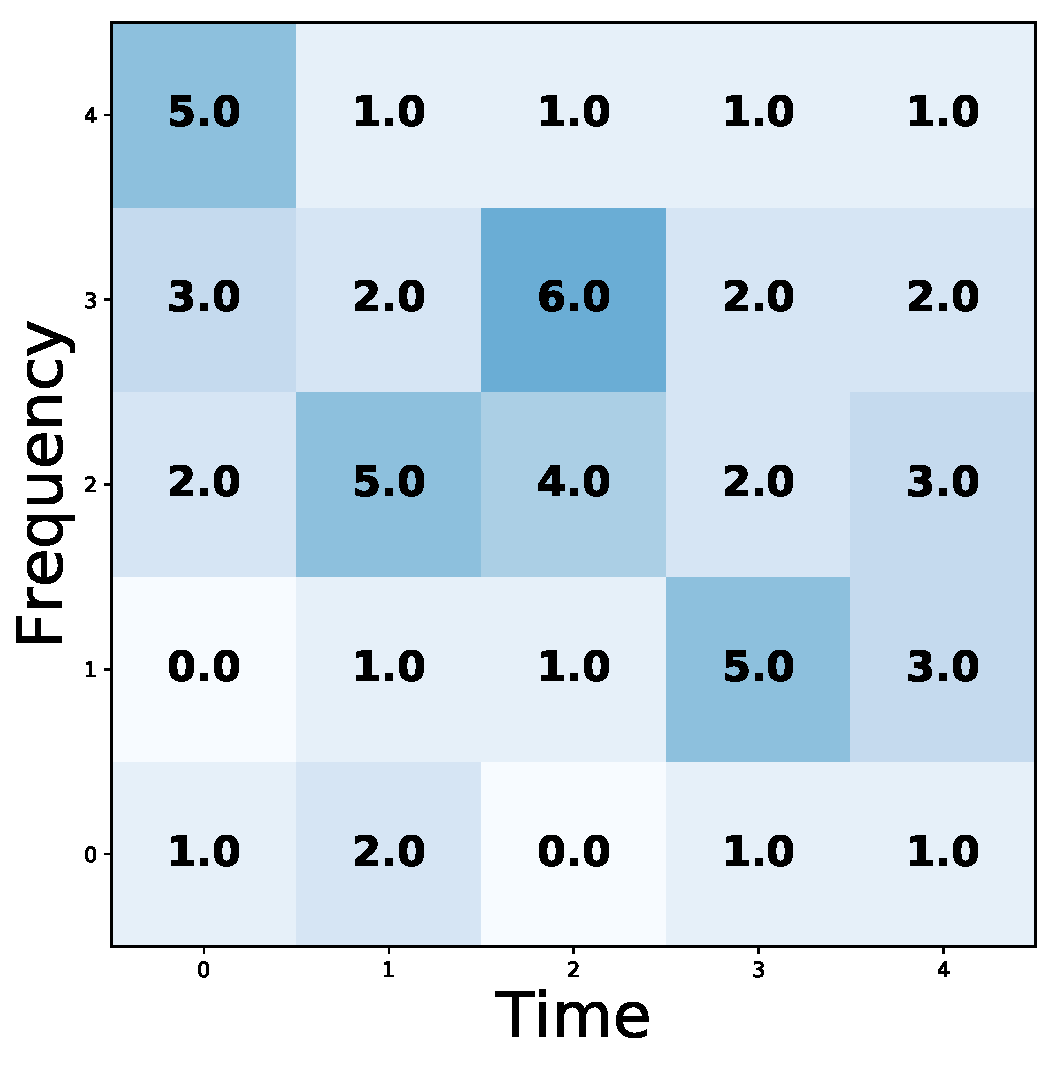
\includegraphics[width=0.8\columnwidth]{vit_data.pdf}
\caption{The input data}
\label{viterbi:plot:data}
\end{subfigure}

\begin{subfigure}[h]{0.8\columnwidth}
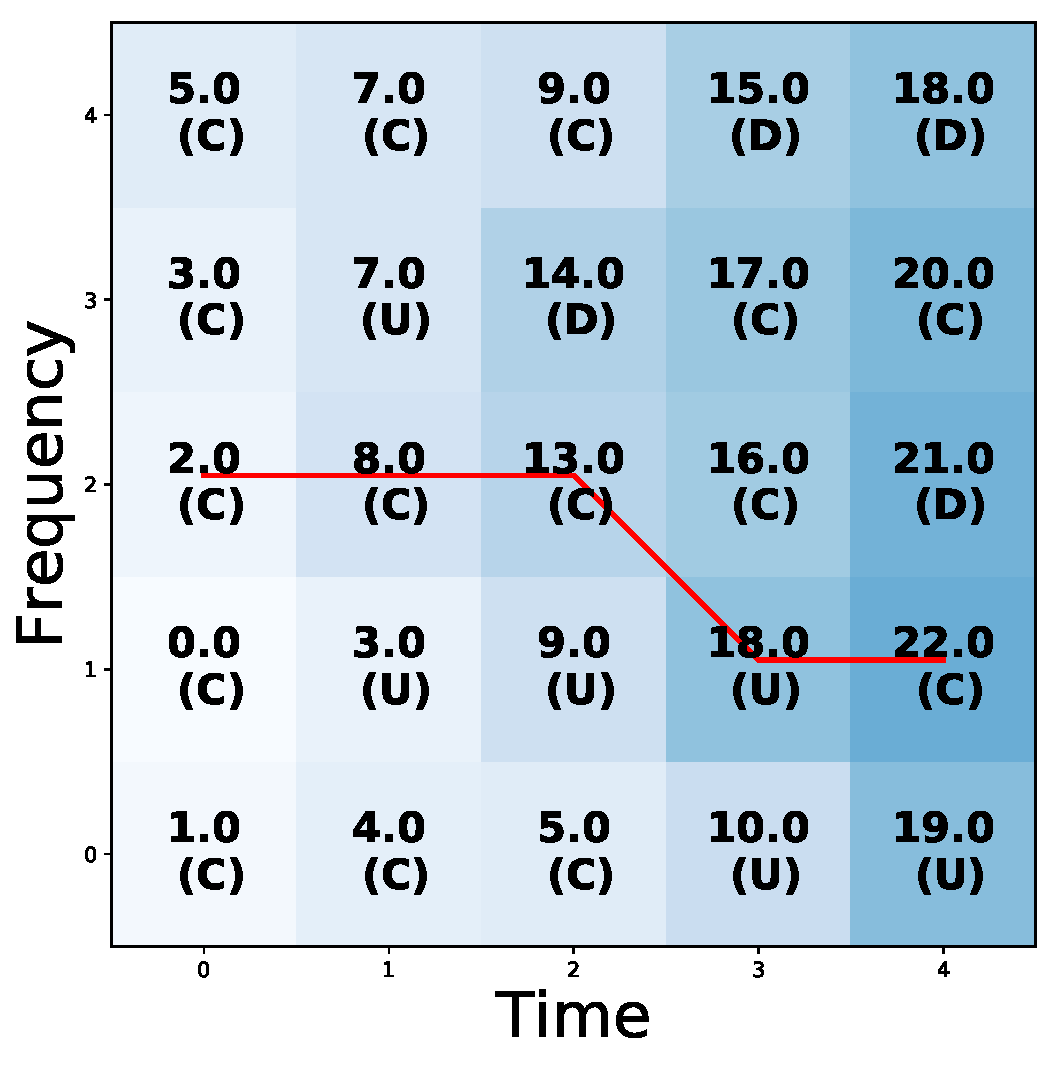
\includegraphics[width=0.8\columnwidth]{vit_prob.pdf}
\caption{The log-probabilities, jumps, and most probable path}
\label{viterbi:plot:likelihood}
\end{subfigure}

\caption{ Fig.~\ref{viterbi:plot:data} shows
the observed data, i.e the log-likelihood values $C_{j,k}$. Fig.~\ref{viterbi:plot:likelihood} shows the calculated
log-probabilities $V_{j,k}$. $A_{j,k}$ is shown in parentheses, where the \ac{UCD}
components correspond to $i= [-1,0,1]$ respectively. The red line shows the
path that gives the maximum probability. The transition matrix for the \ac{UCD} jumps is $[0,1,0]$ and corresponds to the un-normalised prior
log-probabilities of these jumps occurring.}
\label{viterbi:plots}
\end{figure}

\begin{description}
%
% Initialisation
%
\item[Initialisation] The two parts of Eq.~\ref{viterbi:maxtracklog},  $\log p(\nu_0)$ and $\log p({\bm x_0} \mid \nu_0)$, must be computed before the main recursive part of the algorithm can start. Therefore, the initialisation section (lines 5--8) in Alg.~\ref{viterbi:single:algorithm} calculates the first column in the lower panel of Fig.~\ref{viterbi:plots}. A priori, there is no preferred initial frequency, so we take the log-prior $\log p(\nu_{0,k})$ to be uniform over the complete frequency range. As a result, this is does not affect the maximisation for any jump, therefore, can be omitted from the calculation. We then use the pre-calculated log-likelihood values $C_{0,k}$ to fill the track probabilities $V_{0,k}$.  There is no previous position to jump from in this case, so the transition probabilities are irrelevant and $A_{0,k}$ are set to zero.
%
% Iteration
%
\item[Iteration] The main part of the calculation is the sum in Eq.~\ref{viterbi:maxtracklog}. Lines 11--16 in Alg.~\ref{viterbi:single:algorithm} calculate the most probable tracks that end at each frequency bin for each segment by using
    \begin{equation} \label{viterbi:single:vitsum}
    V_{j,k} = \max_{i}({C_{j,k} }+ T_{i} + V_{j-1,k+i}),
    \end{equation}
    where $i$ is the size and direction of the jump. For example, in Fig.~\ref{viterbi:plots} columns 1--4 are calculated in order using Eq.~\ref{viterbi:single:vitsum}, where it maximises over three possible previous positions in frequency. These positions are the frequency bins \ac{UCD} of the current position. The size and direction of the jump, $i$, which gives the maximum probability is then saved to $A_{j,k}$. These are shown in parentheses below the log-probabilities in Fig.~\ref{viterbi:plots} where \ac{UCD} correspond to values of $i = [-1,0,1]$ respectively.
%
% Identification
%
\item[Identification] The final stage of the algorithm identifies the most probable track. This is done by initially finding the highest log-probability values in the final time segment, $\max_k(V_{N-1,k})$ (line 19 in Alg.~\ref{viterbi:single:algorithm}). In the lower panel of Fig.~\ref{viterbi:plots} this is located at position $j,k = 4,1$ with $V_{4,1} = 22$. To find the track which corresponds to this, the values in $A_{jk}$ are followed backwards from this position (lines 20--21). For example, in Fig.~\ref{viterbi:plots} the final position is $j,k = 4,1$ and $A_{j,k} = \rm{Center} = 0$, this means that at the previous segment the most probable track was at position $j,k = 4-1,1+0 = 3,1$. At this time $A_{3,1} = R = 1$, therefore, the next track element is at $j,k = 3-1,1+1 = 2,2$. This then continues until $j=0$ whereupon these retraced positions constitute the most probable track, highlighted in red in Fig.~\ref{viterbi:plots}.
%
\end{description}

%
% mention the limitations - only returns max track.
%
The most probable track is the one traced backwards from the highest probability final segment frequency position. However, tracks can also be traced back from any of the end-frequency positions, returning the most probable track conditional on a given final position. Such tracks should not be confused with the being equal to the second, third, fourth, etc. most probable tracks. Information regarding the rankings and properties of all possible tracks (excluding the most probable and conditionally most probable tracks) is lost during the maximisation procedures computed at each stage in the algorithm --  a necessary consequence of the algorithm's speed and efficiency.

%%%%%%%%%%%%%%%%%%%%%%%%%%%%%%%%%%%%%%%%%%%%%%%%%%%%%%%%%%%%%%%%%%%%%%%%%
%%%%%%%%%%%%%%%%%%%%%%%%%%%%%%%%%%%%%%%%%%%%%%%%%%%%%%%%%%%%%%%%%%%%%%%%%
\section{\label{viterbi:multidet}Multiple detectors}
%%%%%%%%%%%%%%%%%%%%%%%%%%%%%%%%%%%%%%%%%%%%%%%%%%%%%%%%%%%%%%%%%%%%%%%%%
%
% introduce what multidetector means
%
If there are $Q$ detectors operating simultaneously we have $Q$ sets of data which can be combined appropriately to provide input to the Viterbi search described above. We must also modify the allowed transitions encoded within the transition matrix to take account of the extra prior constraints that are now available.

%
% Doppler shift at each detector
%
The received instantaneous frequency of a given astrophysical signal will be nearly the same for all ground-based \ac{GW} detectors, and our
algorithm should be sensitive to tracks that show this consistency in
frequency. However there \emph{will} be small differences between the frequencies measured at detectors that are not co-located, due to differential Doppler shifts caused by Earth rotation. As a result the signal could fall in different frequency bins at each detector.

\iffalse
To sufficient accuracy, the difference in frequency $\Delta f^{(1,2)}$ seen by two detectors ($1$ and $2$), is simply
%
\begin{equation}
\label{viterbi:multidet:doppler}
\Delta f^{(1,2)} = \frac{({{\bm v}^{(1)}} -{{\bm v}^{(2)}})\cdot{\bm \theta}}{c} f_0,
\end{equation}
%
where ${\bm v}_a$ is the velocity of detector $a$ in an inertial reference frame, $\bm \theta$ is a unit vector in the direction of the source and $f_0$ is the instantaneous signal frequency in the reference frame. The maximum difference would occur for two detectors on the equator separated by 180 degrees of longitude and for a source located in the equatorial plane, giving
%
\begin{equation}
\label{viterbi:multidet:doppler:diff}
\Delta f_{\rm max}  \approx 3.1\times 10^{-6} f_0.
\end{equation}
%
For a signal frequency of 200\,Hz the largest possible instantaneous difference in frequency between detectors is therefore $6.2\times 10^{-4}$\,Hz.  Our standard 1800\,s-long \acp{SFT} have a frequency bin-width of $5.6\times 10^{-4}$\,Hz, making this difference significant. As a result it is not enough to simply enforce that the signal tracks follow identical paths in the two detectors and we must allow some level of flexibility on the scale of $\pm 1$ frequency bin.~\chris{I find this paragraph a bit too specific to our analysis choices. We don't have to state the SFT length here. We can simply point out that you can tune the SFT length to give you differing probability distributions on your transition matrix elements. We've chosen to only 1800 sec SFTs and focus on 200\,Hz and therefore use 3 possibilities (UCD) but we could have used a different SFT length and frequency giving us any number of possible jumps. I think that we should make things easy for ourselves and state that we only ever consider 3 possibilities and then you simply tune the SFT length to your frequency spread.}
\fi

%
% Continue algorithm explanation
%
To account for these small differences in signal tracks in each detector, we reference the observed tracks to a third (pseudo) detector located at the centre of the Earth which would be insensitive to Earth spin. The signal frequencies in each real detector are then allowed to vary within a certain number of frequency bins from the track in the reference detector. In the examples that follow, we only consider the possibilities that the track in each real detector is no more that one frequency bin away from the reference track. We can tune the length of the \acp{SFT} to ensure this is a valid assumption.
As well as differences in signal frequency, due to antenna patterns and other effects, the measured signal amplitude may differ between the detectors. In the following example we assume that the signal has the same amplitude in each detector, however, in Sec.~\ref{viterbi:las} we discuss the case where they differ.

We will now show how the algorithm in Sec.~\ref{viterbi:single} can be modified to handle a two-detector network (i.e., $Q=2$),  however any number of detectors can easily be accommodated. In the two detector case the joint probability of two (real) tracks, $\nu^{(1)}$ and $\nu^{(2)}$, and the geocentric track $\nu$, given the data, is
%
\begin{equation}
\begin{split}
p(\nu,\nu^{(1)},\nu^{(2)} | D^{(1)},D^{(2)}) \propto p(\nu)p(\nu^{(1)},\nu^{(2)} | \nu) \\
p(D^{(1)} | \nu^{(1)})p(D^{(2)} | \nu^{(2)}),
\end{split}
\end{equation}
%
where $D^{(1)}$ and $D^{(2)}$ represent the data from the two detectors. The
main difference between this and that described in Sec.~\ref{viterbi:single} is
that the track probabilities $V_{j,k}$ are stored for the geocentric
pseudo-detector. The main iterative calculation (defined for the single
detector case in Eq.~\ref{viterbi:single:vitsum}) now becomes
%
\begin{equation}
\label{viterbi:multidet:vitsum}
  V_{j,k} = \max_{i,l,m}({C}^{(1)}_{j,k+l} + {C}^{(2)}_{j,k+m} + T_{i,l,m} +V_{j-1,k+i}),
\end{equation}
%
where ${C}^{(1)}$ and ${C}^{(2)}$ refer to the log-likelihoods in detectors 1 and 2 respectively and the transition matrix $T$ is an $n_1\times n_2 \times n_3$ matrix, where $n_1$ dimension refers to the jump from the previous time step, $n_2$ and $n_3$ refer to the relative frequency positions in each real detector. The transition matrix is now three-dimensional and holds the prior log-probabilities of $p(\nu)$ and $p(\nu^{(1)},\nu^{(2)} | \nu)$.  We now need to maximise over three indices: $i,l$ and $m$. The index $i$ refers to the size and direction of the jump at the geocentre (as before). The indices $l$ and $m$ refer to the number of frequency bins by which the two real tracks deviate from the geocentre track. For example, if the most probable track in the geocentred detector is in bin $j,k = 5,12$ and the values of $i,l,m = 0,-1,1$, then detector 1 is in position $j,k={5,11}$ and detector 2 is in position $j,k={5,13}$ and the geocentred track was in the position $j,k={4,12}$ at the previous time step. As a result, the track at the geocentre is only affected by Doppler modulations from the Earth's orbit whereas the tracks in the real detectors include Doppler modulations from the Earth's spin.

%
% More details on the doppler constraints
%
At every time step the frequency bin position for each real detector is forced to be within $n_l$ or $n_m$ bins of the track in the geocentred detector, where $n_l$ and $n_m$ depend on how much each detector could possibly be Doppler shifted. As mentioned previously, we only consider the case where $n_l=1$ and $n_m = 1$,  allowing the track from each real detector to be at most one frequency bin away from the geocentred track position. While we tune the \ac{SFT} length to keep this condition for different frequencies, it is also possible to tune the values of $n_l$ and $n_m$ to get a similar effect.
%
% how do we do this in practice?
%
The implementation of the multi-detector algorithm is similar to the single detector case described in Sec.~\ref{viterbi:single}.  However in the single detector case there is only a single variable to be maximised over for each time-frequency bin. This variable is the frequency jump from the position in the previous segment. For the multi-detector case there are at least three variables to be maximised over: the probability of the jump, $i$, at the geo-centre and the probability of the signal being in the surrounding positions in each on $Q$ real detectors, $l,m,\dots$. The values of $i,l,m, \dots$ are then saved to $A_{j,k}$ and are ultimately used to reconstruct the most probable consistent tracks in each real detector.

%
%  algorithm explanation
%
As in Sec.~\ref{viterbi:single}, there are three main sections: Initialisation, iteration, and the identification. For the multi-detector case each element is modified as follows.

\begin{description}
% first step calculation
\item[Initialisation] The first-row calculation (lines 5--8) in Alg.~\ref{viterbi:single:algorithm}, are now modified to additionally maximise over the real detector track positions $l$ and $m$. For each time-frequency bin the maximum sum of the log-likelihoods is saved together with the frequency locations of the corresponding tracks in the real detectors. The index $i=0$ is kept constant as there is no previous position.

% all other steps calculation
\item[Iteration] To process the subsequent time segments, lines 13--14 in Alg.~\ref{viterbi:single:algorithm} are modified to account for two (or more) detectors. Line 13 of Alg.~\ref{viterbi:single:algorithm} is changed to calculate Eq.~\ref{viterbi:multidet:vitsum}, the log-probability of a track at the geocentre ending in bin $j,k$ given that signal is in the real detector positions of $j,k+l$ and $j,k+m$. Line 14 is then modified so that $A_{j,k}$ stores the jump values, $i$, and the real detector positions, $l$ and $m$, which returned the highest probability.

% finding the most probable track
\item[Identification] The most probable track is identified in the same way as for the single detector case, first by finding the maximum value in the final time step of $V_{j,k}$ (line 19 in Alg.~\ref{viterbi:single:algorithm}). The track at the geocentre can then be found by iteratively following the jump values stored in $A_{j,k}$ back from this position. The track in each of the real detectors is determined by using the values of $l$ and $m$ indices also stored in $A_{j,k}$ to find the relative position of the track in each real detector compared to the geocentre.
%
\end{description}

This method can be extended to more than two detectors by including additional datasets and expanding the corresponding number dimensions of the maximisation procedures in the iterative steps.

%%%%%%%%%%%%%%%%%%%%%%%%%%%%%%%%%%%%%%%%%%%%%%%%%%%%%%%%%%%%%%%%%%%%%%%%%
%%%%%%%%%%%%%%%%%%%%%%%%%%%%%%%%%%%%%%%%%%%%%%%%%%%%%%%%%%%%%%%%%%%%%%%%%
\section{\label{viterbi:memory} Memory}
%%%%%%%%%%%%%%%%%%%%%%%%%%%%%%%%%%%%%%%%%%%%%%%%%%%%%%%%%%%%%%%%%%%%%%%%%
%
% general idea of memory
%
In this section we extend the basic Viterbi algorithm to improve its sensitivity to non-stochastic signals where there is some knowledge of its frequency evolution.
We do this by including a form of `memory' and this extension applies to both the single and multiple-detector cases.
Rather than considering only the previous step in our decision-making process, we now include the previous $m+1$ steps and expand the transition matrix to include these values.
A memory of $m=0$ therefore corresponds to the methods described in previous sections.
With a non-zero memory the transition matrix can a-priori make certain sequences of jumps more probable and assign different prior probabilities for these jump sequences e.g., `up then centre' may be less preferable to `centre then centre'.
As a result we can increase the chance of the most probable track matching an expected astrophysical signal.
In a single detector search with a memory of $m=1$, if we only allow \ac{UCD} transitions, then for every frequency bin we save 3 values. These are proportional to the log-probabilities of a track coming from a \ac{UCD} bin in the previous time step, where the maximisation is over the corresponding \ac{UCD} bins two time steps back.
Eq.~\ref{viterbi:multidet:vitsum} then is then modified to,
%
\begin{equation}
\label{viterbi:memory:stat}
V_{j,k,s} = \max_{h} ({C}_{j,k} + T_{s,h} +  V_{j-1,k+s,k+s+h}),
\end{equation}
%
where $s$ and $h$ refer to the \ac{UCD} jumps at the time step $j-1$ and $j-2$ respectively.  Similar to the previous two sections, the algorithm is split into three parts: initialisation, iteration, and the track identification:

\begin{description}
% initialisation
\item [Initialisation] The initialisation process needs to populate the first $m+1$ steps before the main iteration can start. At the first time step, the elements $V_{0,k,s}$ are set to the log-likelihoods $C_{0,k}$ as in Sec.~\ref{viterbi:single}.  There is no previous time step, so the element $s$ is not relevant. At the second time step, $V_{1,k,s}$ is calculated using Eq.~\ref{viterbi:memory:stat}, where there is no maximisation over $h$, it is assumed to be $0$, or a center jump. As there is no data before $j=0$, the maximisation at this point will always return the jump which has the largest prior probability, which in this case is a center jump. Therefore, the maximisation returns the same value for all frequency bins and can be set to a center jump.

%Iteration
\item [Iteration] For all following time steps the values for each element of $V_{j,k,s}$ in Eq.~\ref{viterbi:memory:stat} are calculated. This quantity is proportional to the log-probability of the track ending in time-frequency bin $j,k$, which was in the previous position of $j-1,k+s$. The corresponding value of $h$ that maximised the log-probability of the track is recorded in $A_{j,k,s}$.

%Identification
\item [Identification] The most probable track is identified in a similar way to the non-memory cases, by finding the highest-valued last element, $V_{N-1,k,s}$. The values of $s$ and $h$ are then followed back to find the most probable track. As an example, let us assume the most probable track finishes in bin $j,k,s = 10,5,0$, where the value of $m$ is $A_{10,5,0} = 1 = \rm{up}$. The previous position is then $j,k,s=10-1,5+s,m =10-1,5+0,1=9,5,1$ with a value $A_{9,5,1} = 0 = \text{Center}$, and the next track position is $j,k,s=9-1,5+1,0=8,6,0$ etc. The values of $j,k$ along this track describes most probable path.
%
\end{description}

The number of elements over which one must search increases rapidly with memory length, and has a strong impact on the computational cost of the analysis. For the single detector Viterbi approach the number of calculations made is $3 \times N \times M$ if we only allow \ac{UCD} jumps, where $N$ and $M$ are the number of time are frequency bins respectively. When memory is included this increases to $3^{m+1} \times N \times M $.

%%%%%%%%%%%%%%%%%%%%%%%%%%%%%%%%%%%%%%%%%%%%%%%%%%%%%%%%%%%%%%%%%%%%%%%%%
%%%%%%%%%%%%%%%%%%%%%%%%%%%%%%%%%%%%%%%%%%%%%%%%%%%%%%%%%%%%%%%%%%%%%%%%%
\section{\label{viterbi:sumdata}Summed input data}
%%%%%%%%%%%%%%%%%%%%%%%%%%%%%%%%%%%%%%%%%%%%%%%%%%%%%%%
%
% describe what we propose to do with summed SFT power
%
In this section we outline a method of incoherently-summing a set of \acp{SFT} to increase the \ac{SNR} of a signal in a segment. To be more precise, we actually sum the log-likelihoods, i.e. the quantity in Eq.~\ref{viterbi:periodogram}. We can write the new summed set of data $F_j$ as,
%
\begin{equation}
F_j = \sum_{i}^{N_s}C_{i,k}
\end{equation}
%
where $N_s$ is the number of \acp{SFT} to sum together and the log-likelihood $C(\nu_{i,k})$ is defined in Eq.~\ref{viterbi:periodogram}.
We can see this is possible by looking at Eq.~\ref{viterbi:single:likelihood}, where we can use the product of likelihoods,
%
\begin{equation}
\begin{split}
p(D \mid \nu) &\propto p(x_1,x_2 \ldots x_n \mid \nu) \\
&\propto p(x_1 \mid \nu) \ldots p(x_n \mid \nu) \\
&\propto \exp{\left( \sum_i C_{j,k}\right)}.
\end{split}
\end{equation}
%
If the data contains gaps where the detector was not observing, then we fill the gaps in the power spectrum with a constant value which is the expectation value of the log-likelihood. The procedure of filling in the gaps of the data is completed before any summing.  Therefore, the data should have the same mean regardless of how much real data is in each sum. In the examples that follow, we sum the \acp{SFT} over the length of one day.

The main motivation for summing the data is to increase the \ac{SNR} of a signal in the segments. The risk is that a signal can move between adjacent frequency bins during a day. To reduce this risk, we choose the frequency bin width such that it is more likely that a signal will be contained within a single frequency bin that cross a bin edge. In practise, to ensure that this is true, the segment or \ac{SFT} length and the number of segments which are summed can be tuned for each search. As well as increasing the \ac{SNR}, summing over one day should average out the antenna pattern. This means that the log-likelihood value in any bin should be more similar between detectors, however, there is still some variation due to the sky localisation and polarisation.

This also has two main effects on the transition matrix, the first is that as each segment of data is now one day long, a jump between frequency bins is far more likely, therefore, the transition matrix elements are modified to account for this. The second is that as the data is averaged over one day, the signal should remain is the same frequency bin between detectors, therefore, there is no longer a need for the multi-dimensional transition matrix described in Sec.~\ref{viterbi:multidet}.

The volume of the data is also reduced by a factor of $1/N_s$, therefore, the time taken for the algorithm to run is also reduced by the same factor.

%%%%
% EXTRA INFO NOT INCULDED AT THE MOMENT
%%%%%%%
\iffalse

Using the same example in Sec.~\ref{viterbi:multidet}, we have two detectors that are at opposite sides of the earth on the equator.
A signal in the equatorial plane at 150\,Hz will have a spread of frequency of $\Delta f = 3.1 \times 10^{-6} \times 150 \; \rm{Hz} = 4.7 \times 10^{-4} \; \rm{Hz}$.
This is less than the bin width of our 1800\,s \acp{SFT} which is $5.6 \times 10^{-4} \; \rm{Hz}$.
Therefore, over the course of one day the signal should spend most of its time within one \ac{SFT} frequency bin.
For the real \ac{LIGO} detectors this will be less due to their locations, therefore, we can assume that the signal stays within one frequency bin for the duration of a day.
This then allows us to sum the \acp{SFT} over one day, i.e. as we have 1800\,s long \acp{SFT}, we can add every 48 together.

\fi
%%%%%%%

%%%%%%%%%%%%%%%%%%%%%%%%%%%%%%%%%%%%%%%%%%%%%%%%%%%%%%%%%%%%%%%%%%%%%%%%%
%%%%%%%%%%%%%%%%%%%%%%%%%%%%%%%%%%%%%%%%%%%%%%%%%%%%%%%%%%%%%%%%%%%%%%%%%
\section{\label{viterbi:las}Line-aware statistic}
%%%%%%%%%%%%%%%%%%%%%%%%%%%%%%%%%%%%%%%%%%%%%%%%%%%%%%%%%%%%%%%%%%%%%%%%%
%
% what is the line aware statistic
%
The multiple-detector algorithm described in Sec.~\ref{viterbi:multidet} returns the most probable track of a common signal assumed to be in Gaussian noise. As a consequence the algorithm will return large values of the log-likelihood even if there are inconsistent values of \ac{SFT} power between the detectors, either from non-Gaussian noise or because the signal is not equally strong in the two detectors. However a signal with unequal power in the two detectors is more likely to be a non-Gaussian instrumental line than an astrophysical signal. The line-aware statistic described in this section is designed to make the search more robust to such instrumental artefacts within realistic non-Gaussian data whilst maintaining sensitivity to astrophysical signals.

%
% More detail on what this is applied to
%
For most of the analysis examples presented here we use data which is the incoherent sum of 30-minute normalised \acp{SFT} over a day (described in more detail in Sec.~\ref{viterbi:sumdata}). As a result the effects of the detector antenna patterns and of differential Doppler shifts are significantly reduced, and any signal should have a broadly similar summed log-likelihood in the same frequency bin in each detector. The statistic can then be modified such that we expect a similar log-likelihood in each detector.

We first consider the model of Gaussian noise with no signal present. Within
a single summed segment, the likelihood of Gaussian noise at
frequency $\nu$ is given by a $\chi^2$ distribution,
%
\begin{equation}
\label{las:central}
p(F_j|\nu_j,M_{\text{N}},I) = \frac{1}{2^{d/2}\Gamma(d/2)}F_j^{d/2 - 1}\exp{\left\{
\frac{F_j}{2}\right\}}
\end{equation}
%
where $F_j$ is the frequency domain power summed over sub-segments within a single day, as described in Sec.~\ref{viterbi:sumdata} and  $d$ is the number of degrees of freedom,  equal to twice the total number of summed SFTs.  $M_{\rm{N}}$ represents the model that the data is simply Gaussian noise. In the presence of a signal (model $M_{\text{S}}$), the power should follow a non central $ \chi^2 $ distribution in which the non-centrality parameter $\lambda$ is the square of the \ac{SNR}, $(\lambda = \rho_{\rm{opt}}^2 )$, i.e.
%
\begin{equation}
\label{las:noncentral}
\begin{split}
p(F_j|\nu_j,\lambda,M_{\text{S}},I) = \frac{1}{2} \exp{\left\{ -\frac{F_j+\lambda}{2}\right\}} \left( \frac{F_j}{\lambda} \right)^{d/4 - 1/2} \\
I_{d/2 -1}\left( \sqrt{\lambda F_j}\right).
\end{split}
\end{equation}
%
If a signal is present we therefore expect the \ac{SFT} powers in both detectors to follow Eq.~\ref{las:noncentral}.  Assuming for the moment that the noise variance is the same in both, we can determine the evidence for model $M_{\text{S}}$ by marginalising over $\lambda$,
%
\begin{equation}
\label{las:signal}
\begin{split}
p(F^{(1)}_{j},F^{(2)}_{j} \mid \nu_j,M_{\rm{S}},I) = \int_0^{\infty}  p(\lambda,w_{\rm_S}) \\
p(F^{(1)}_{j}|\nu_j,\lambda,M_{\text{S}},I)p(F^{(2)}_{j}|\nu_j,\lambda,M_{\text{S}},I) d\lambda.
\end{split}
\end{equation}
%
We set the prior on $\lambda$ to be an exponential distribution of width $w$, this is done somewhat arbitrarily as we expect the majority of signals to have a low \ac{SNR}. This distribution follows,
\begin{equation}
\label{las:prior}
p(\lambda,w) = \exp\left( \frac{-\lambda}{w}\right).
\end{equation}

On the other hand, if an instrumental line is present in one of the detectors we expect to see signal-like power in that detector and noise-like power in the other.  The evidence for this `line' model ($M_{\text{L}}$) is therefore
%
\begin{equation}
\label{las:signal}
\begin{split}
p(F^{(1)}_{j},F^{(2)}_{j} \mid \nu_j,M_{\rm{L}},I) = \int_0^{\infty}  p(\lambda,w_{\rm_L}) \\
\left[ p(F^{(1)}_{j}|\nu_j,M_{\rm{N}},I)p(F^{(2)}_{j}|\nu_j,\lambda,M_{\rm{S}},I) \right. \\
\left. + p(F^{(1)}_{j}|\nu_j,\lambda,M_{\rm{S}},I)p(F^{(2)}_{j}|\nu_j,M_{\rm{N}},I)\right]d\lambda ,
\end{split}
\end{equation}
%
The third option to consider is the simple case of approximately Gaussian noise in both of the detectors,
%
\begin{equation}
\label{las:noise}
\begin{split}
p(F^{(1)}_{j},F^{(2)}_{j} \mid \nu_j,\lambda,M_{\rm{G}},I) = p(F^{(1)}_{j} \mid \nu_j,M_{\rm{G}},I) \\
p(F^{(2)}_{j} \mid \nu_j,M_{\rm{G}},I) .
\end{split}
\end{equation}
The posterior probability of model $M_{\text{GL}}$, which contains the probability of Gaussian noise or Gaussian noise with a line in one detector, (taken as mutually exclusive) is
\begin{equation}
\begin{split}
p(M_{\rm{GL}} \mid F^{(1)}_{j},F^{(2)}_{j},\nu_j ,I) = p(M_{\rm{G}} \mid F^{(1)}_{j},F^{(2)}_{j},\nu_j ,I) \\
+p(M_{\rm{L}} \mid F^{(1)}_{j},F^{(2)}_{j} ,\nu_j, I),
\end{split}
\end{equation}
where we assume that $M_{\rm{G}}$ and $M_{\rm{L}}$ are mutually exclusive.

%
We can now find the posterior odds ratio for the presence of a signal over noise or a line,
\begin{widetext}
\begin{equation}
\label{viterbi:odds}
\begin{split}
O_{\rm{SGL}}(F^{(1)}_{j},F^{(2)}_{j}\mid\nu_j) &=  \frac{p(M_{\rm{S}} \mid F^{(1)}_{j},F^{(2)}_{j} ,\nu_j)}{p(M_{\rm{GL}} \mid F^{(1)}_{j},F^{(2)}_{j},\nu_j)}
= \frac{p(M_{\rm{S}} \mid F^{(1)}_{j},F^{(2)}_{j} ,\nu_j)}{p(M_{\rm{G}} \mid F^{(1)}_{j},F^{(2)}_{j} ,\nu_j) +p(M_{\rm{L}} \mid F^{(1)}_{j},F^{(2)}_{j} ,\nu_j)}\\
&=\frac{p(M_{\rm{S}})p(F^{(1)}_{j},F^{(2)}_{j} \mid M_{\rm{S}},\nu_j)}{p(M_{\rm{G}})p(F^{(1)}_{j},F^{(2)}_{j}\mid M_{\rm{G}},\nu_j) + p(M_{\rm{L}})p(F^{(1)}_{j},F^{(2)}_{j}\mid M_{\rm{L}},\nu_j) } \\
&= \frac{p(F^{(1)}_{j},F^{(2)}_{j} \mid M_{\rm{S}},\nu_j)p(M_{\rm{S}})/p(M_{\rm{G}})}{p(F^{(1)}_{j},F^{(2)}_{j}\mid M_{\rm{G}},\nu_j) + p(F^{(1)}_{j},F^{(2)}_{j}\mid M_{\rm{L}},\nu_j)p(M_{\rm{L}})/p(M_{\rm{N}}) }
\end{split}
\end{equation}
\end{widetext}
In practice it is convenient to use the log odds ratio,
\begin{equation}
\begin{split}
\label{viterbi:logodds}
\log\left[ O_{\rm{SGL}}(F^{(1)}_{j},F^{(2)}_{j})\right] &=  \log\left[ p(F^{(1)}_{j},F^{(2)}_{j} \mid M_{\rm{S}}) \right] \\
&- \left[ \log\left( p(F^{(1)}_{j},F^{(2)}_{j}\mid M_{\rm{G}}) \right. \right. \\
&\left.\left.+  p(F^{(1)}_{j},F^{(2)}_{j}\mid M_{\rm{L}})p(M_{\rm{L}})/p(M_{\rm{G}})\right) \right]
\end{split}
\end{equation}
As we are only interested in the maximum of $\log\left[ O_{\rm{SGL}}(F^{(1)}_{j},F^{(2)}_{j})\right]$, the factor $\log\left[ p(M_{\rm{S}})/p(M_{\rm{G}})\right]$ can be dropped from the expression.


In this version of the Viterbi algorithm, rather than storing a value proportional to the log-probabilities as in Sec.~\ref{viterbi:multidet}, here we store a value proportional to the log-odds ratio.
Here we take the log-odds ratio defined in Eq.~\ref{viterbi:logodds}, which is the log-odds of a signal having a similar power in each detector, and add the log-prior odds $p(\bm{\nu} \mid M_S)/(p(\bm{\nu} \mid M_N) + p(\bm{\nu} \mid M_L))$ which is the log-prior or any particular track. By assuming that the track transitions for the line and noise model are equally probable for any jump, we set the denominator of the prior-odds is a constant $b$.
This then means Eq.~\ref{viterbi:multidet:vitsum} is modified to,
\begin{equation}
\begin{split}
\label{lineaware:stat}
\hat{V}_{i,j} = \max_{k,l,m}\left(T_{k,l,m} + b + V_{i-1,j+k}   \right. \\
 + \left.  \log\left[O_{\rm{SGL}}\left(F^{(1)}_{j},F^{(2)}_{j}\right)\right]\right),
\end{split}
\end{equation}
%
where $\hat{V}$ refers to a log-odds ratio.
The maximised statistic now has three tuneable parameters: the width, $w_S$ in Eq.~\ref{las:prior}, on the prior for a signal \ac{SNR} squared, $p_{\rm S}(\lambda)$, the width, $w_L$ of the prior in the case of a line, $p_{\rm L}(\lambda)$, and the ratio of the prior on the line and noise models, $p({M_{\rm L}})/p({M_{\rm G}})$.  These parameters are optimised for each search, where we initially estimate the \ac{SNR} of a signal we hope to be sensitive to in each time slice, then use this as a guide for the width of the signal prior. This is then repeated for an expected line \ac{SNR} and this is used for the width of the line prior. The ratio of line and noise models runs in the range 0 to 1, we set this limit as we do not expect an instrumental line to be as likely as Gaussian noise in any particular frequency bin.

\section{Line aware statistic with unequal noise floors}

In this section we modify the line aware statistic above to account for differences in sensitivity and duty cycle of the detectors.

\chapter{Convolutional neural networks}

\section{Layers}

\subsection{Neurons}

\subsection{Convolutional layers}

\subsection{Max pooling layers}

\subsection{Fully connected layers}

\subsection{Activation functions}

\subsection{loss functions}

\section{Training}

\section{CW search}

\subsection{Viterbi Maps}

\subsection{SFTs}

\subsection{Viterbi map and SFTs}

%!TEX root = main.tex
\chapter{SOAP searches}

\section{Gaussian Noise}

\section{S6}

\subsection{S6 MDC}

\subsection{S6}

\section{O1}

\subsection{Astrophysical}

\subsection{Instrumental Lines}

\section{O2}

\subsection{Astrophysical}

\subsection{Instrumental Lines}

\section{O3}

\subsection{Astrophysical}

\subsection{Instrumental Lines}


\chapter{Armadillo}

\section{Control systems}

\section{}

\appendix

%\backmatter  % Turn off chapter numbering
% I assume that the bibliography is assembled by hand.
% Change the file if you use bibtex or something like that.
\bibliography{references.bib}

\end{document}
